\documentclass[11pt]{article}
\usepackage[margin=1in]{geometry}
\usepackage[french]{babel}
\usepackage[T1]{fontenc}
\usepackage[utf8]{inputenc}
\usepackage{graphicx}
\usepackage{array}
\usepackage{tikz}
\usetikzlibrary{arrows.meta, positioning}
\usepackage{placeins}
\usepackage{float}

\usepackage{bookmark}
\RequirePackage{tabularx}
\usepackage{array}
\usepackage{tabularx}
\usepackage{booktabs}
\usepackage{xcolor}
\usepackage{hyperref}
\usepackage{geometry}
\usepackage{pdflscape}
\usepackage{longtable}
\usepackage{ltablex}
\usepackage{amsmath}
\usepackage{listings}
\usepackage{svg}

\usepackage{xcolor}

\lstdefinestyle{CStyle}{
  language=C,
  basicstyle=\ttfamily\small,
  keywordstyle=\color{blue!70!black}\bfseries,
  stringstyle=\color{green!40!black},
  commentstyle=\color{gray!80}\itshape,
  numbers=left,
  numberstyle=\tiny\color{gray},
  stepnumber=1,
  numbersep=8pt,
  showstringspaces=false,
  tabsize=2,
  breaklines=true,
  breakatwhitespace=true,
  frame=single,
  framerule=0.4pt,
  rulecolor=\color{black!30},
  backgroundcolor=\color{black!2},
  captionpos=b
}



\setlength{\parindent}{0pt}

\begin{document}

\begin{titlepage}
\thispagestyle{empty}
\centering

\vspace*{0.6cm}

\begin{minipage}[c][5.4cm][c]{0.43\textwidth}
  \centering
  \fbox{\parbox[c][4.8cm][c]{0.92\linewidth}{\centering
    
\includegraphics[width=0.9\linewidth]{assets/logo_polytech.png}
  }}
\end{minipage}
\hspace{0.8cm}
\begin{minipage}[c][5.4cm][c]{0.43\textwidth}
  \centering
  \fbox{\parbox[c][4.8cm][c]{0.92\linewidth}{\centering
    
\includegraphics[width=0.82\linewidth]{assets/logo_st_mars.png}
  }}
\end{minipage}

\vspace{1.5cm}

{\fontsize{28}{32}\selectfont\bfseries RAPPORT TECHNIQUE FIN DE PROJET\par}
\vspace{0.55cm}
{\Large Projet transversal n\textsuperscript{o}4\par}
\vspace{0.45cm}
{\LARGE\bfseries Collecteur de données animalières\par}

\vspace{1.2cm}

{\large Équipe projet :\par}
{Davy Clark, Ewen Le Callet, Joris Menard, Jules Noumba, Xueying Xu\par}

\vspace{0.55cm}

{\large Client :\par}
{Xavier Leprevost -- Élu de la mairie de Saint-Mars-du-Désert\par}

\vspace{0.55cm}

{\large Encadrants :\par}
{Abdelhakim Saadane et Antoine Goullet\par}

\vspace{0.55cm}

{\large Date :\par}
{09/03/2026\par}

\vfill

{\large Année universitaire 2025--2026\par}

\end{titlepage}

\clearpage
\section*{Remerciements}
\addcontentsline{toc}{section}{Remerciements}
Nous tenons à remercier l'ensemble des personnes ayant contribué à la réalisation de ce projet transversal. 
Nous remercions particulièrement nos encadrants, Abdelhakim Saadane et Antoine Goullet, pour leur accompagnement,
leurs conseils méthodologiques et leur disponibilité tout au long de l'année universitaire 2025--2026.

Nous remercions également notre client, Xavier Leprevost, élu de la mairie de Saint-Mars-du-Désert,
pour sa confiance, la clarté de ses besoins et la qualité des échanges durant le développement du
\textit{collecteur de données animalières}.

\clearpage
\tableofcontents

\clearpage
\listoffigures
\addcontentsline{toc}{section}{Table des figures}

\clearpage
\section*{Glossaire}
\addcontentsline{toc}{section}{Glossaire}
\begin{description}
  \item[WP] Un Work Package (WP) est une unité de travail dans un projet. Il regroupe un ensemble cohérent de tâches, d’objectifs et de livrables.

\end{description}


\newpage

\section{Introduction}
Le projet \textbf{Collecteur de données animalières} s'inscrit dans le cadre du projet transversal 2025--2026 mené
par des étudiants de Polytech Nantes en collaboration avec la mairie de Saint-Mars-du-Désert.

L'objectif principal est de concevoir une solution permettant de collecter, structurer et exploiter des données
relatives à la faune locale, afin d'améliorer le suivi du territoire et d'appuyer la prise de décision.

Ce rapport technique présente le contexte du projet, les besoins exprimés par le client, les choix techniques
retenus, ainsi que l'avancement des travaux réalisés par l'équipe. Par ailleurs, la structuration en lots de travail
s'inspire des bonnes pratiques de gestion de projet recommandées dans la littérature\cite{PMBOK2021}. Par ailleurs, la structuration en lots de travail
s'inspire des bonnes pratiques de gestion de projet recommandées dans la littérature\cite{PMBOK2021}.

\section{Présentation, contexte et spécifications}
\subsection{Présentation de l’entreprise}
\subsection{Contexte général}
\subsection{Présentation du sujet de projet et Cahier des Charges}
\subsection{Etat de l'art}



\section{Liste des Work-Packages : Objectifs, Solution, Validation}

Parler de la décomposition des WP, sous WP etc

\subsection{WP 1.1 — Détection de mouvement et mesure de température (responsable : Jules Noumba)}
\subsubsection{Rappel des objectifs}
Détailler objectifs et liste des taches.
\subsubsection{Solution envisagé}
Travail théorique et recherches
\subsubsection{Tests et Validation}
Tests et validation de vos taches.




\subsection{WP 1.2 — Gestion des échanges données et du microcontrôleur (responsable : Nolan Buchet)}

\subsubsection{Rappel des objectifs}

Pour recontextualiser le projet et les objectifs de ce Work Package, le WP 1.2 fait partie du Work Package 1 qui 
est dédié à la conception et au développement du système de collecte de données animalières. Le WP 1.2 se concentre 
spécifiquement sur la gestion des échanges de données entre les différents composants du système, ainsi que sur 
l'intégration et la programmation du microcontrôleur qui servira de cerveau central pour le projet. De plus celui-ci 
s'occupera de la partie énergétique du module, ainsi que de la partie stockage des données collectées.
\\

Voici la liste des tâches qui seront réalisées dans le cadre de ce WP :
\begin{itemize}
    \item Tâche 0 ( Équipe ) : Choix du microcontrôleur et de la carte SD
    \item Tâche 1 : Gestion du stockage des données collectées
    \item Tâche 2 ( hors WP ) : Gestion de la luminosité pour WP 1.3
    \item Tâche 3 : Gestion de l'horodatage et de la localisation du module
    \item Tâche 4 : Définition d'un automate pour la gestion globale du module
    \item Tâche 5 : Gestion de l'alimentation du module
    \item Tâche 6 : Intégration des modules ( prototypage )
    \item Tâche 7 : Développement d'une architecture électrique
    \item Tâche 8 : Création d'un PCB pour le module
    \\
\end{itemize}

Pour chacune des tâches réalisées ci-dessus, il y a eu une phase de test réalisée, ainsi qu'en amont une phase de concertation avec 
l'équipe du WP afin que les solutions envisagées soient en adéquation avec les besoins du projet.
\\

Certaines tâches de ce module ne sont pas dans l'ordre de conception, comme la tâche 4 ou 5 qui ont été en constante évolution 
durant tout le projet. Et certaines tâches non essentielles, mais logiques, comme l'optimisation du code ou le rapport / documentation, ont 
été réalisées en parallèle de la conception du module.
\\

\subsubsection{Tâche 0 : Choix du Microcontrôleur}

\subsubsection*{Solution envisagée}

À la suite d’une phase de recherche ( benchmark du début de projet ) concernant le contrôleur à utiliser pour ce projet, nous avons identifié deux solutions susceptibles 
de répondre à nos besoins : l’ESP32 et le Raspberry Pi Zero.
\\

Pour rappel, les besoins principaux concernant le contrôleur étaient les suivants :
\\

\begin{center}
\renewcommand{\arraystretch}{1.3}
\begin{tabularx}{0.9\textwidth}{>{\bfseries}l|X}
\toprule
\textbf{Critère} & \textbf{Description} \\
\midrule
Consommation énergétique & Minimiser la consommation pour un usage sur batterie. \\ 
Performances & Garantir une puissance suffisante pour le traitement des données. \\ 
Stockage & Disposer d’une capacité suffisante pour enregistrer temporairement les mesures locales et la photographie. \\ 
Système & Offrir un environnement logiciel simple avec facilité sur les outils de développement utilisés. \\ 
Interfaces & Proposer des entrées/sorties adaptées aux capteurs et modules externes. \\ 
Connectivités & Intégrer ou supporter le Wi-Fi, le Bluetooth ou d'autres moyens de communication. \\ 
Prix & Rester dans une gamme de coût compatible avec le budget du projet. \\ 
\bottomrule
\end{tabularx}
\end{center}

Ces critères nous ont permis de comparer plusieurs solutions techniques lors de la phase de benchmark.
\\

Les critères suivants ont été considérés lors du choix final du microcontrôleur :
\begin{itemize}
    \item Architecture matérielle
    \item Connectivité
    \item Consommation énergétique
    \item Nombre et type de GPIO
    \item Facilité de développement
    \item Coût global
    \\
\end{itemize}

À l’issue de l’analyse comparative réalisée entre l’ESP32 et le Raspberry Pi Zero, le choix s’est porté sur l’ESP32 comme microcontrôleur 
principal pour le collecteur de données animalières. Ce choix est motivé par plusieurs facteurs clés. Tout d’abord, sa faible consommation
énergétique constitue un avantage décisif pour une utilisation sur batterie dans un environnement isolé. L’ESP32 peut fonctionner 
plusieurs jours, voire semaines, en mode basse consommation, ce qui garantit une autonomie optimale sur le terrain.
\\

Ensuite, son intégration native du Wi-Fi et du Bluetooth simplifie la conception matérielle et réduit le besoin de modules externes, 
tout en permettant la transmission sans fil des données et la configuration à distance du système.
\\

Enfin, son coût réduit et sa disponibilité sur le marché en font une solution économique et accessible, sans compromis majeur sur 
les performances nécessaires au projet. En revanche, il est à noter que le Raspberry Pi Zero offre une puissance de calcul et une
mémoire supérieures, mais celles-ci sont jugées excessives au regard des besoins du projet et pénalisantes en termes de consommation 
énergétique et de gestion logicielle.
\\

En conclusion, l’ESP32 répond pleinement aux exigences du projet en matière de consommation, de connectivité et de simplicité de 
déploiement, ce qui en fait la solution la plus adaptée pour le collecteur de données animalières.
\\

\noindent\textit{Notes :}  
Un document détaillé présentant l’analyse comparative entre l’ESP32 et le Raspberry Pi Zero, ainsi que les critères de sélection, 
a été rédigé.

\subsubsection{Tâche 1 : Gestion du stockage des données collectées}

\subsubsection*{Rappel des objectifs}

Commençons par la tâche 1, qui est la gestion du stockage des données collectées. Pour cette tâche, il a été décidé d'utiliser 
une carte SD ( par cahier des charges ) pour stocker les données collectées, notamment les métadonnées et les images. La carte SD offre une grande 
capacité de stockage, ce qui est essentiel pour notre projet. De plus, les cartes SD sont relativement faciles à interfacer avec un 
microcontrôleur, ce qui facilite l'intégration dans notre système. Enfin, celle-ci est facilement accessible pour les utilisateurs, 
ce qui permet une récupération facile des données collectées.
\\

Donc nous avons utilisé un module de carte SD utilisable via le moyen de communication SPI, qui est un protocole de communication série rapide 
et efficace. Le microcontrôleur peut ainsi envoyer des commandes à la carte SD pour lire et écrire des données de manière rapide et fiable.
Le module utilisé est un module personnel ( \texttt{AZDelivery SPI Reader} ), celui-ci a été choisi au début du projet car aucune
commande n'était envisageable de la part du département ou du client.
\\

\begin{figure}[H]
    \centering
    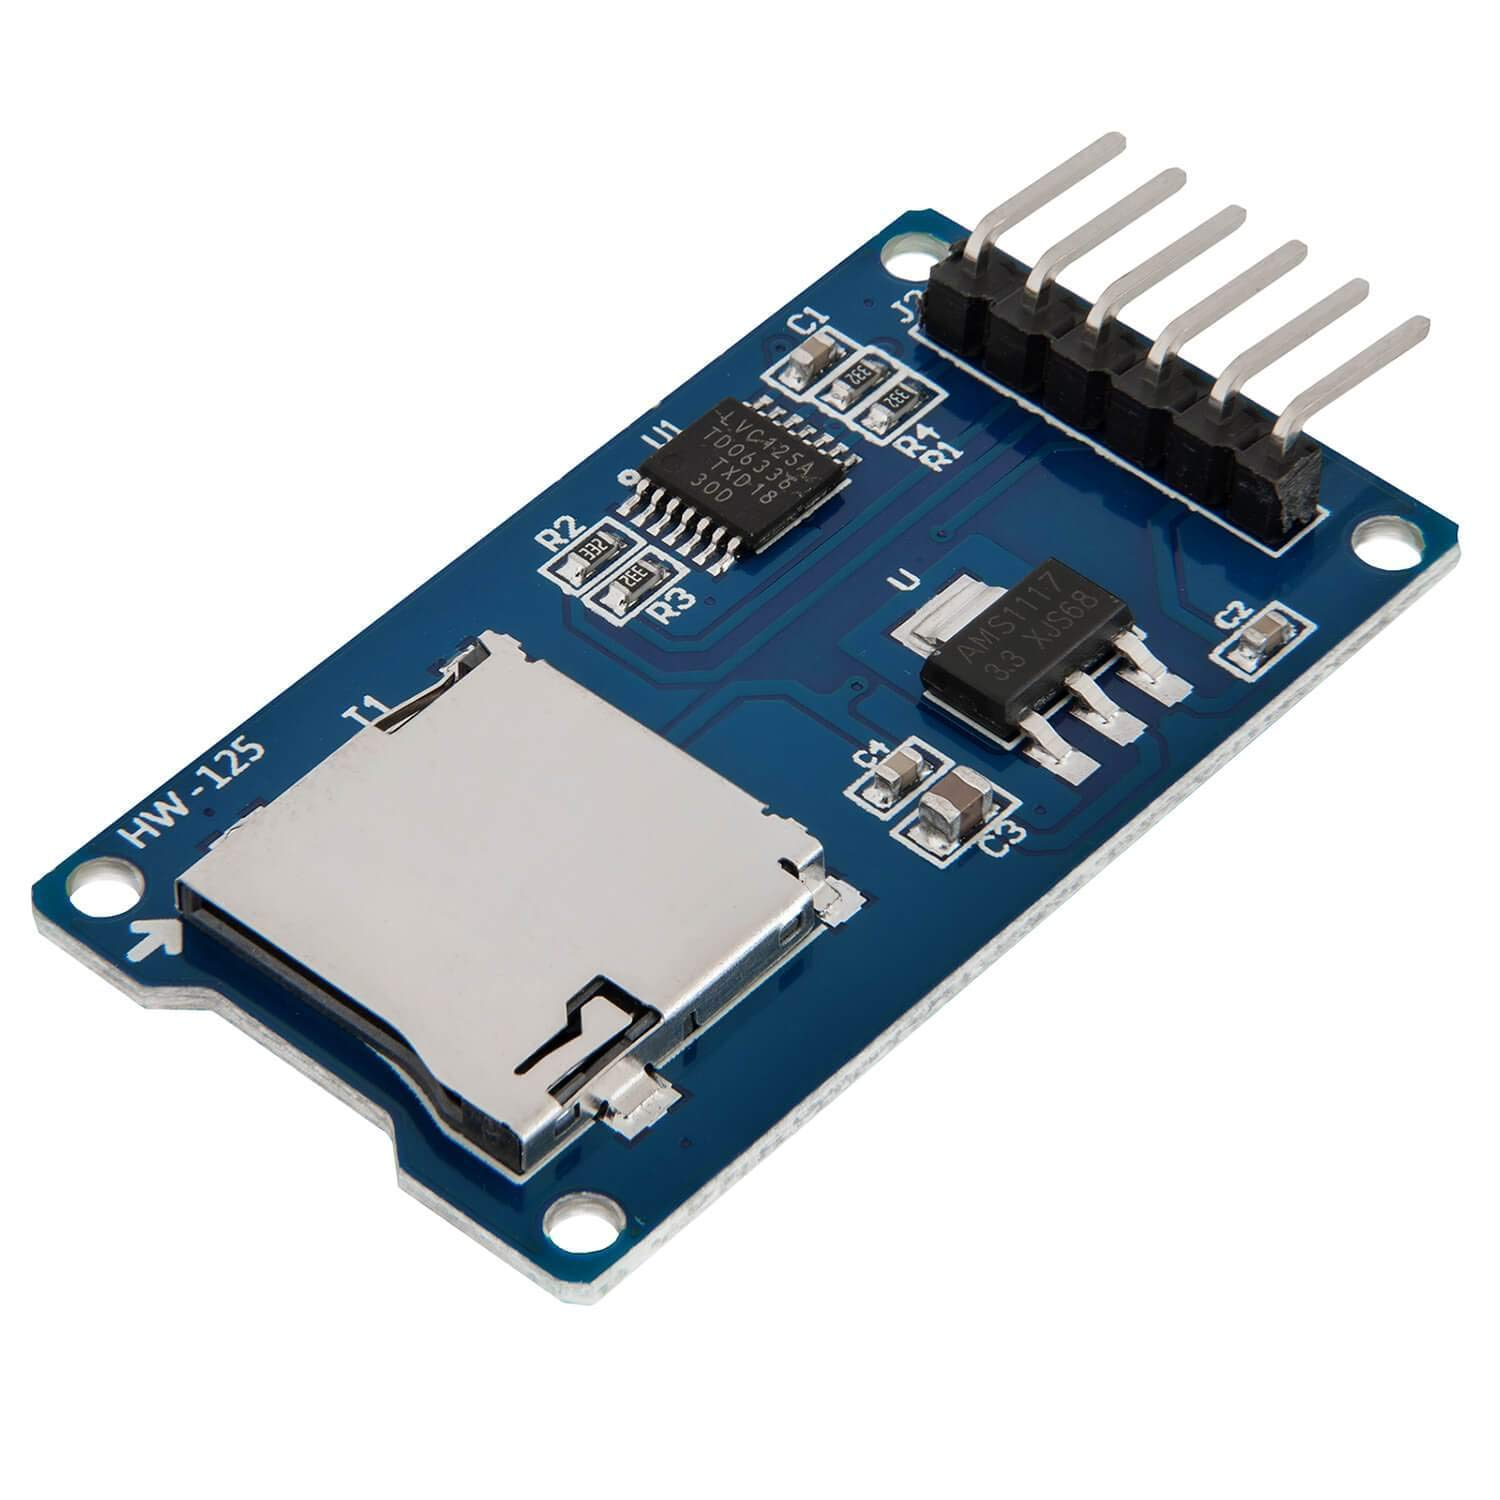
\includegraphics[width=0.4\textwidth]{Images/WP1_2/Tache_1/ModuleSD.jpg}
    \caption{Module de carte SD utilisé pour le projet}
\end{figure}

\subsubsection*{Solution envisagée}

Pour utiliser le module, nous avons connecté notre ESP32 à ce module en liaison SPI, en utilisant les broches suivantes :
\begin{itemize}
    \item MOSI ( Master Out Slave In : Écriture ) : GPIO 13
    \item MISO ( Master In Slave Out : Lecture ) : GPIO 12
    \item SCK ( Serial Clock ) : GPIO 14
    \item CS ( Chip Select ) : GPIO 15
    \item VCC : 5V
    \item GND : GND
    \\
\end{itemize}

Nous utiliserons le module HSPI de l'ESP32 pour la communication SPI, qui permet des vitesses de transfert élevées.
Voici un exemple de communication en SPI pour décrire le moyen de communication entre l'ESP32 et la carte SD. 

\begin{figure}[H]
    \centering
    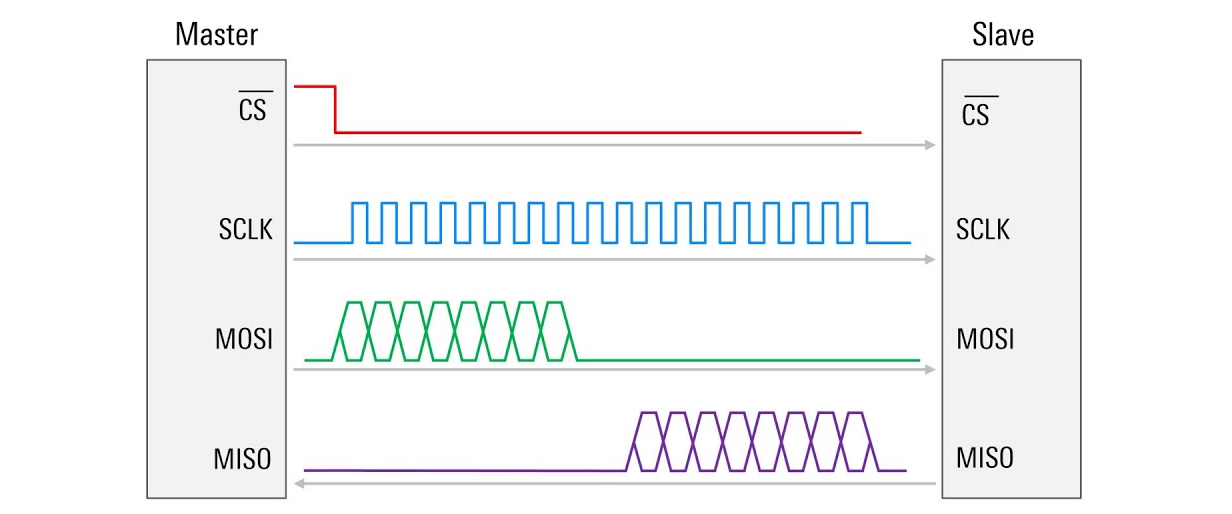
\includegraphics[width=0.8\textwidth]{Images/WP1_2/Tache_1/SPI.png}
    \caption{Module de carte SD utilisé pour le projet}
\end{figure}


Pour utiliser ce module, une librairie toute faite a déjà été développée, qu'il a suffi d'implémenter dans notre projet pour pouvoir 
utiliser la carte SD. Cette librairie est la librairie \texttt{SD.h} qui est une librairie standard pour la gestion des cartes SD avec 
les microcontrôleurs Arduino et ESP32. Elle offre des fonctions pour initialiser la carte SD, lire et écrire des fichiers, 
et gérer les répertoires. Nous l'avons utilisée pour créer notre propre bibliothèque visant à simplifier l'utilisation de cette carte, 
notamment pour le WPBis qui est dédié à la gestion de la transmission des données collectées.
\\

\subsubsection*{Tests et Validation}

Pour la phase de test, nous avons juste réalisé un test afin de savoir si nous pouvions écrire un fichier texte sur la carte SD,
en donnant comme nom de fichier les métadonnées ( comme température, humidité, etc ), afin de simuler un buffer de réception d'images avec 
les données correspondantes.
\\

Voici un exemple de code utilisé pour ce test :

\begin{lstlisting}[style=CStyle, caption={Exemple utilisation module SD}, label={lst:sd_exemple}]
#include <SD_PIEGE.h>

void setup()
{ 
    initSD(); 
    
    // Temperature_Humidite_Latitude_Longitude_Heure_Minute_Seconde
    String filename = "20_60_47-2833012_1-5152623_10-30-30.txt"; 
    
    File file = SD.open(filename, FILE_WRITE); 
    
    // Exemple de donnees JPEG 
    uint8_t image[] = {0xFF, 0xD8, 0xFF, 0xE0, 0x00, 0x10, 0x4A, 0x46}; 
    
    file.write(image, sizeof(image)); 
    file.close(); 
}
\end{lstlisting}

\begin{figure}[H]
    \centering
    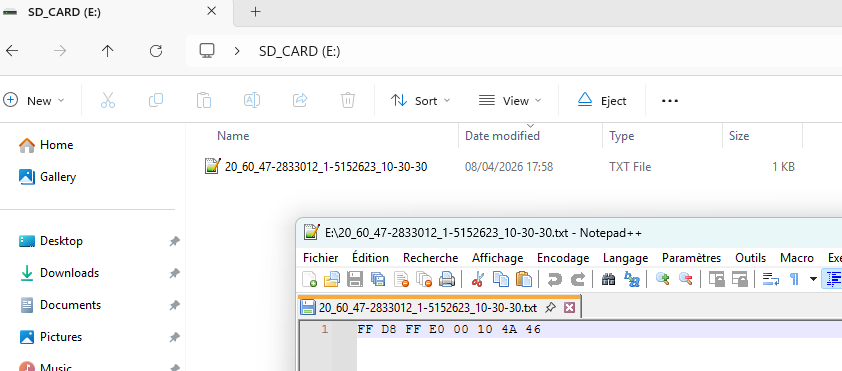
\includegraphics[width=0.8\textwidth]{Images/WP1_2/Tache_1/Result_SD.png}
    \caption{Résultat du test d'écriture sur la carte SD}
\end{figure}

\subsubsection{Tâche 2 : Hors WP : Gestion de la luminosité pour WP 1.3}

\subsubsection*{Rappel des objectifs}

Pour cette partie nous avons décidé de nous séparer de notre WP afin d'aider le 
WP 1.3 qui est dédié à la gestion de la caméra, notamment pour la partie de 
la luminosité. En effet, la luminosité est un facteur important pour la 
prise de vue des images, car d'après notre cahier des charges, nous voulions
prendre des photographies de jour comme de nuit. 
\\

Avoir la possibilité de connaître la luminosité de l'environnement nous permettrait
de pouvoir allumer une source de lumière ( comme des LED infrarouges ) pour pouvoir
capturer des éléments de nuit.
\\

\subsubsection*{Solution envisagée}

Pour cela nous avons décidé d'ajouter un capteur de luminosité ( une photorésistance ( LDR )) 
afin de capturer la luminosité de l'environnement. Ce capteur est un composant électronique 
qui change de résistance en fonction de la quantité de lumière. C'est un capteur très simple à mettre
en œuvre et à interfacer avec un microcontrôleur comme l'ESP32. En mesurant la résistance de la 
photorésistance, nous pouvons déterminer la luminosité ambiante et ajuster le comportement de notre système.
\\

Pour connaître la résistance de ce capteur, nous utilisons un montage de diviseur de tension, 
qui nous permet de convertir la résistance variable de la photorésistance en une tension mesurable par l'ESP32.
Voici un schéma de ce montage :
\\

\begin{figure}[H]
    \centering
    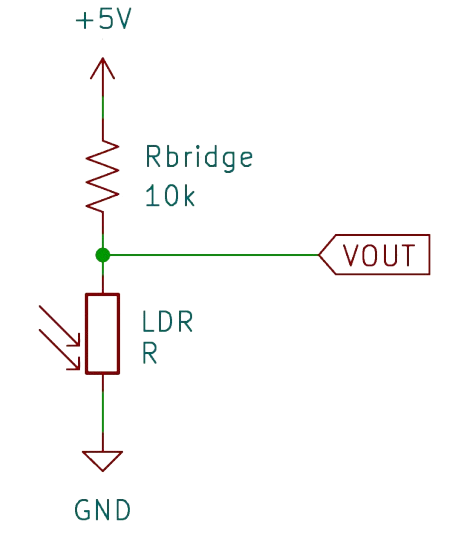
\includegraphics[width=0.4\textwidth]{Images/WP1_2/Tache_2/ldr_sche.png}
    \caption{Schéma du montage de diviseur de tension pour la photorésistance}
\end{figure}

Dans ce montage, la photorésistance ( LDR ) est connectée en série avec une résistance fixe ( R1 ).
Lorsque la lumière frappe la photorésistance, sa résistance change, ce qui modifie la tension de sortie ( Vout ) du diviseur de tension.
En mesurant cette tension de sortie avec l'ESP32, nous pouvons calculer la résistance de la photorésistance et ainsi déterminer la luminosité ambiante.
\\

\[
    R_{LDR} = (( R_{serie} * 3.3 ) / Tension_{Vout} ) - R_{serie};
\]


À partir de la documentation technique de la LDR, nous pouvons facilement retrouver la valeur
de la luminosité ( en LUX ) à partir de la résistance, en utilisant la courbe suivante :
\\

\begin{figure}[H]
    \centering
    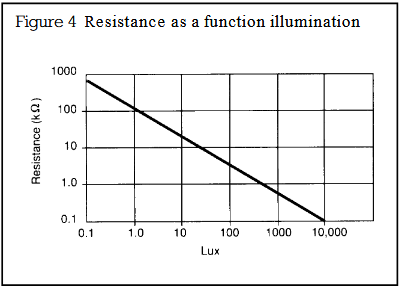
\includegraphics[width=0.6\textwidth]{Images/WP1_2/Tache_2/CourbeLDR.png}
    \caption{Courbe de résistance en fonction de la luminosité pour la photorésistance}
\end{figure}

\[
    Lux = (\frac{1000}{Resistance})^{1.4}   
\]

\subsubsection*{Tests et Validation}

Pour la phase de test de cette LDR, nous avons tout simplement effectué 
plusieurs mesures avec des taux de luminosité différents, en utilisant une lampe, un chiffon, un rideau, etc. 
pour faire varier la luminosité, et en mesurant la tension de sortie du diviseur de tension.
\\

Pour lire la valeur numérique nous avons tout simplement utilisé la fonction \texttt{analogRead()} de l'ESP32, 
qui nous permet de lire la tension de sortie.
\\

Voici un exemple de code utilisé pour ce test :

\begin{lstlisting}[style=CStyle, caption={Exemple utilisation LDR}, label={lst:ldr_exemple}]
#define LDR_PIN 34 // Broche analogique pour la LDR
#define RESISTOR_BRIDGE 10000 // Resistance diviseur de tension 

void setup() 
{
    Serial.begin(115200); 
}

void loop() 
{
    // Calcul de la tension ( ADC 12 bits )
    ldrValue = (analogRead(LDR_PIN) * 3.3) / (1.0 * 4095.0);

    // Calcul de la reistance 
    float resistance = (( RESISTOR_BRIDGE * 3.3 ) / ldrValue ) - RESISTOR_BRIDGE;
    
    // Calcul de la luminosite en LUX
    float lux = pow((1000 / resistance), 1.4); 

    Serial.print("LDR Value: ");
    Serial.println(ldrValue); // Affichage de la valeur lue
    
    Serial.print("Resistance: ");
    Serial.println(resistance); // Affichage de la resistance calculee
    
    Serial.print("Luminosite (LUX): ");
    Serial.println(lux); // Affichage de la luminosite calculee

    delay(1000); // Attente d'une seconde avant la prochaine lecture
}
\end{lstlisting}

Avec ce code nous avons pu vérifier que notre capteur LDR fonctionnait comme un luxmètre,
en affichant la valeur de luminosité en LUX dans le moniteur série de l'ESP32. 
Nous avons en même temps vérifié à l'aide d'un luxmètre ( téléphone ) que les valeurs de 
luminosité affichées étaient cohérentes avec les mesures réelles. Malheureusement le téléphone 
utilisant une application, celui-ci n'était pas très précis.
\\

Mais dans l'ensemble, les résultats obtenus étaient cohérents, nous avons obtenu : 
\\

\begin{table}[H]
    \centering
    \footnotesize
    \setlength{\tabcolsep}{3pt}
    \renewcommand{\arraystretch}{1.15}
    \resizebox{\textwidth}{!}{%
    \begin{tabular}{|l|c|c|c|c|c|c|c|c|c|}
        \hline
        & \multicolumn{3}{c|}{\textbf{Theorie (Calcul)}} & \multicolumn{3}{c|}{\textbf{Numerique (Code)}} & \multicolumn{3}{c|}{\textbf{Pratique (Multimetre + Telephone)}} \\
        \cline{2-10}
        & \textbf{Tension} & \textbf{Resistance} & \textbf{Lux} & \textbf{Tension} & \textbf{Resistance} & \textbf{Lux} & \textbf{Tension} & \textbf{Resistance} & \textbf{Lux (PAS FIABLE)} \\
        \hline
        \textbf{Noir (Torchon)} & 0 & 1M & 0,1 & 0 & 1M & 1 & 0 & 17,16M & 0 \\
        \hline
        \textbf{Sombre} &  &  &  & 0,69 & 5668 & 2636 & 0,7 & 5300 & 100 \\
        \hline
        \textbf{Gris} &  &  &  & 2 & 996 & 5413 & 2,13 & 890 & 500 \\
        \hline
        \textbf{Lumiere} &  &  &  & 2,71 & 329 & 7312 & 2,8 & 237 & 1900 \\
        \hline
        \textbf{Flash} & 3,3 & 0,1 & 10000 & 3,3 & 0 & 9820 & 3,22 & 72,3 &  \\
        \hline
    \end{tabular}
    }
    \caption{Comparaison des mesures de luminosite : theorie, calcul numerique et mesures pratiques}
    \label{tab:ldr_comparaison}
\end{table}

Nous avions pour principe de construire notre propre couronne de LED infrarouges, avec ce capteur LDR, afin de pouvoir capturer des
animaux durant la nuit, mais par facilité nous avons décidé d'acheter une couronne de LED infrarouges déjà faite, 
qui s'allume à partir d'une certaine luminosité, ce qui nous a permis de ne pas avoir à gérer l'allumage de ces LED, et de se 
concentrer sur d'autres aspects du projet.
\\

Cette couronne de LED a une détection de luminosité automatique, si le seuil est assez élevé, alors les LED s'allumeront, 
et si le seuil est bas alors les LED seront éteintes, ce principe est aussi géré par une photorésistance, 
mais celle-ci est intégrée dans la couronne de LED, ce qui nous a permis de ne pas avoir à gérer cet aspect et de simplement alimenter ce module.
\\

\begin{figure}[H]
    \centering
    \begin{minipage}[t]{0.48\textwidth}
        \centering
        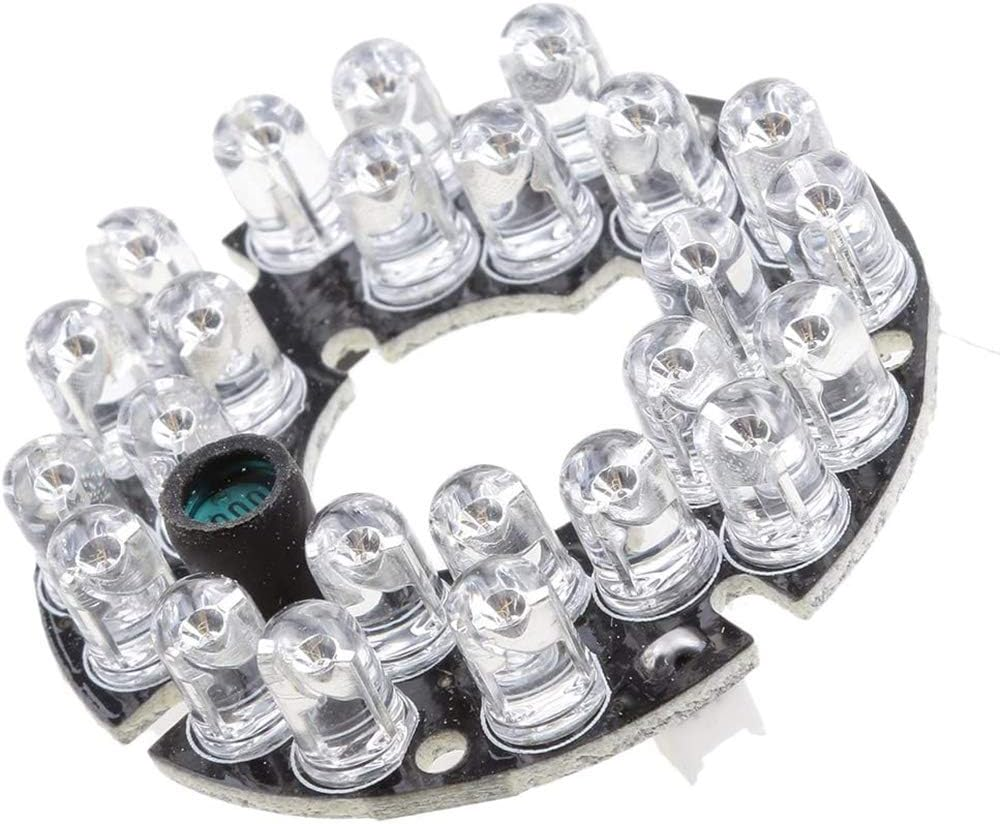
\includegraphics[width=\linewidth]{Images/WP1_2/Tache_2/couronne_1.jpg}
        \par\small Couronne de LED Infrarouge utilisée pour le projet - face avant
    \end{minipage}
    \hfill
    \begin{minipage}[t]{0.48\textwidth}
        \centering
        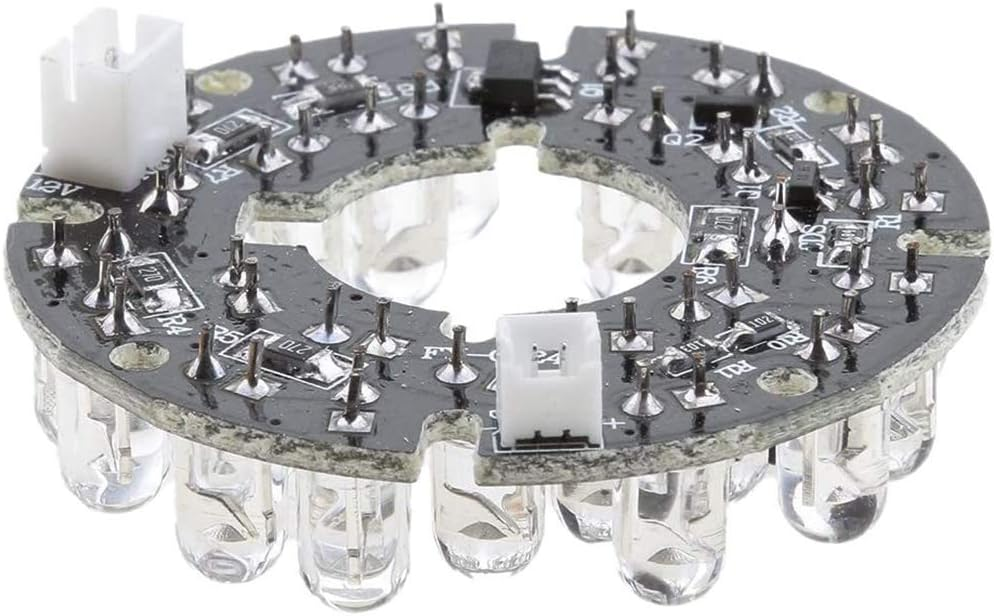
\includegraphics[width=\linewidth]{Images/WP1_2/Tache_2/couronne_2.jpg}
        \par\small Couronne de LED Infrarouge utilisée pour le projet - face arrière
    \end{minipage}
    \caption{Couronne de LED Infrarouge utilisée pour le projet}
\end{figure}

Malheureusement, avec les différents problèmes rencontrés durant le projet, nous n'avons pas pu faire de vrais tests dans la nature afin
de vérifier que nous puissions capturer les animaux de nuit, mais nous avons pu faire des tests en intérieur, en nous prenant en photo
dans le noir.
\\

\subsubsection{Tâche 3 : Gestion de l'horodatage et de la localisation du module}

\subsubsection*{Rappel des objectifs}

Pour cette tâche, nous avons décidé d'ajouter un module GPS afin de pouvoir récupérer la localisation du module, ainsi que l'heure 
grâce à ce module. En effet, les données d'horodatage sont nécessaires pour pouvoir obtenir des statistiques sur le taux
de passage dans la zone en question, et la localisation est nécessaire dans le cas où nous aurions plusieurs modules à déployer, afin 
d'observer les zones de passage.
\\

Nous avons décidé d'utiliser un module GPS personnel ( dans le même cas que pour la carte SD, aucune commande n'était envisageable de 
la part du département ou du client ), qui est un module basique destiné plutôt aux drones FPV.
\\

\begin{figure}[H]
    \centering
    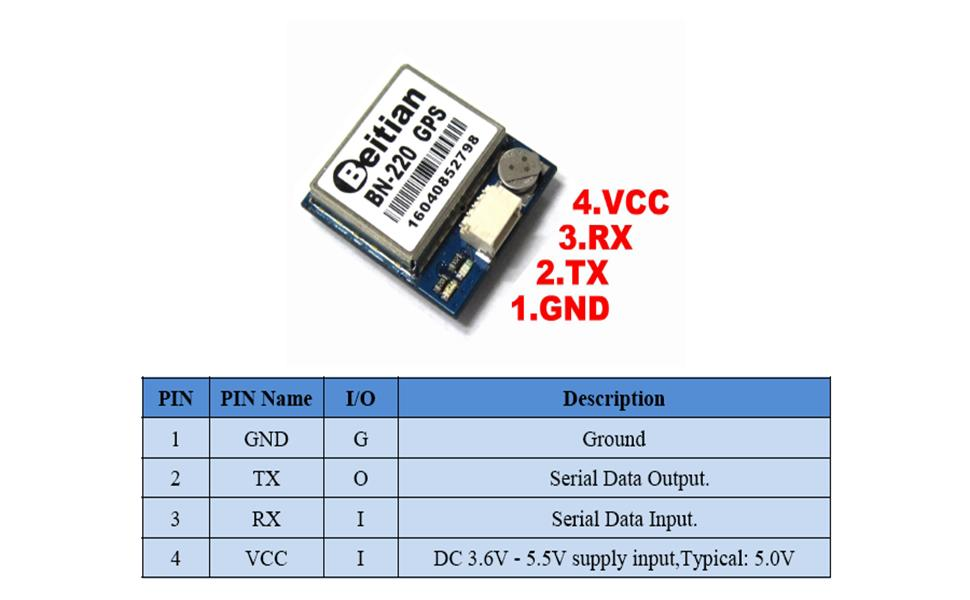
\includegraphics[width=0.8\textwidth]{Images/WP1_2/Tache_3/BN220.jpg}
    \caption{Module GPS utilisé pour le projet}
\end{figure}

\subsubsection*{Solution envisagée - GPS}

Ce module est basé sur une communication Série UART, qui est un protocole de communication simple et largement utilisé pour les modules GPS.
Celui-ci envoie des données de localisation et d'horodatage au format NMEA, qui est un format standard pour les données GPS.
Différentes trames NMEA contiennent différentes informations, telles que la position, la vitesse, l'heure, etc. 
\\

Par exemple, la trame la plus connue est celle de GGA, qui est : 
\\

\begin{figure}[H]
    \centering
    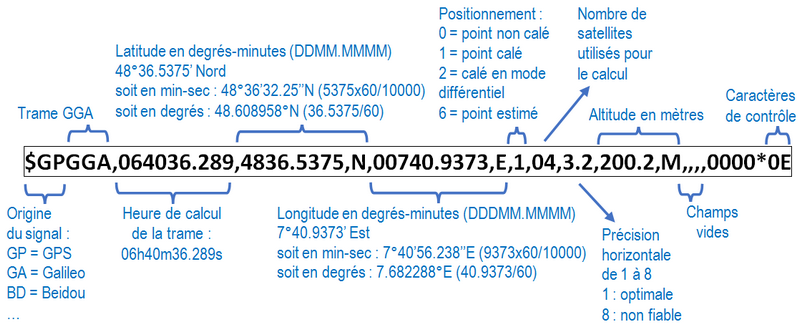
\includegraphics[width=0.8\textwidth]{Images/WP1_2/Tache_3/tramenmea.png}
    \caption{Exemple de trame NMEA envoyée par le module GPS}
\end{figure}

Dans notre cas nous allons utiliser la trame \texttt{GPRMC} :

\begin{figure}[H]
    \centering
    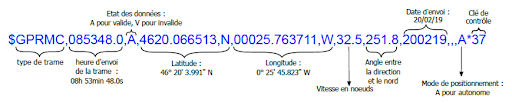
\includegraphics[width=0.8\textwidth]{Images/WP1_2/Tache_3/GPRMC.png}
    \caption{Trame GPRMC utilisée pour récupérer la localisation et l'horodatage}
\end{figure}

Grâce à cette trame, nous allons pouvoir récupérer l'heure ( UTC ), la latitude et la longitude.
\\

Pour l'implémentation de ce module, nous avons créé notre librairie Arduino visant à récupérer les informations que 
nous souhaitons à partir des informations de communication en liaison UART. 
\\

Le principe est simple : nous attendons qu'une trame complète soit arrivée, nous analysons si le caractère de début est bien \texttt{\$GPRMC}, 
et nous analysons les caractères qui sont séparés par des virgules pour récupérer les différentes informations.
À la suite de ça nous avons créé une classe en C permettant de pouvoir récupérer les valeurs directement via une simple fonction, \texttt{get()}.
\\

\subsubsection*{Solution envisagée - RTC}

Pour la partie du GPS nous avons pu voir que nous pouvions récupérer toutes les informations nécessaires à notre projet,
cependant il y avait un problème : le GPS met du temps à capter la localisation car celui-ci dépend de la position des 
satellites, et dans le cas où le module est dans une zone isolée, il peut mettre du temps à capter la localisation.
\\

Une solution était d'utiliser un module RTC ( Real Time Clock ), celui-ci permettrait de continuer à obtenir l'heure sans pour autant
avoir besoin d'utiliser le module GPS, ce qui nous permettrait de gagner du temps sur tout le cheminement de la capture à la transmission.
\\

Un module RTC est un composant électronique qui maintient une horloge en temps réel, même lorsque le microcontrôleur est éteint ou redémarré.
Voici un schéma du principe que nous voulions implémenter : 
\\

\begin{figure}[H]
    \centering
    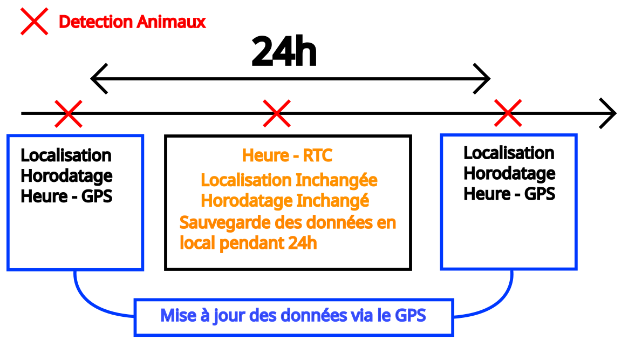
\includegraphics[width=0.8\textwidth]{Images/WP1_2/Tache_3/Schema_GPS.png}
    \caption{Schéma du principe de fonctionnement du module RTC pour maintenir l'heure en temps réel}
\end{figure}

Pour l'implémentation de ce module, nous avons implémenté notre propre librairie qui vise à initialiser le module RTC avec les données du GPS, 
et ensuite, comme pour le GPS, à avoir des fonctions get() pour récupérer les différentes informations de date et d'heure.
\\

Donc après l'implémentation de ce code, nous avons au total 10 données qui sont sauvegardées dans le module RTC, qui sont :
\begin{itemize}
    \item Seconde : String
    \item Minute : String
    \item Heure : String
    \item Jour : String
    \item Mois : String
    \item Année : String
    \item Latitude : char 
    \item Longitude : char 
    \item activation du GPS : bool ( permet de connaître l'activation de la première fois du GPS pour la synchronisation de l'heure )
    \item lastRefreshDay : int ( permet d'enregistrer le jour auquel les métadonnées ont été rafraîchies par le GPS )
\end{itemize}

\subsubsection*{Tests et Validation}

Dans un premier temps nous avons vérifié que nous recevions bien les trames NMEA du module GPS, en affichant les données 
reçues dans le moniteur série de l'ESP32.
\\

\noindent
\begin{minipage}[t]{0.45\textwidth}
\begin{lstlisting}[style=CStyle, caption={Exemple utilisation module GPS}, label={lst:gps_exemple}]
void loop()
{
    gps.update();
    Serial.println("Donnees GPS recues :");

    Serial.print("Latitude: ");
    Serial.println(
        gps.getLatitude());
    Serial.print("Longitude: ");
    Serial.println(
        gps.getLongitude());
    Serial.print("Heure UTC: ");
    Serial.print(
        gps.getHours());
    Serial.print(":");
    Serial.print(
        gps.getMinutes());
    Serial.print(":");
    Serial.println(
        gps.getSeconds());
    Serial.print("Date (JJ/MM/AAAA): ");
    Serial.print(
        gps.getDay());
    Serial.print("/");
    Serial.print(
        gps.getMonth());
    Serial.print("/");
    Serial.println(
        gps.getYear());

    delay(10000); // Attente 10s 
}
\end{lstlisting}
\end{minipage}
\hfill
\begin{minipage}[t]{0.45\textwidth}
\begin{lstlisting}[style=CStyle, caption={Moniteur Série de l'ESP32}, label={lst:moniteur_exemple}]
Donnees GPS recues :
Latitude: 47.2833012
Longitude: 1.5152623
Heure UTC: 10:38:32
Date (JJ/MM/AAAA): 09/04/2026

Donnees GPS recues :
Latitude: 47.2833012
Longitude: 1.5152623
Heure UTC: 10:38:42
Date (JJ/MM/AAAA): 09/04/2026

Donnees GPS recues :
Latitude: 47.2833012
Longitude: 1.5152623
Heure UTC: 10:38:52
Date (JJ/MM/AAAA): 09/04/2026

Donnees GPS recues :
Latitude: 47.2833012
Longitude: 1.5152623
Heure UTC: 10:39:02
Date (JJ/MM/AAAA): 09/04/2026

Donnees GPS recues :
Latitude: 47.2833012
Longitude: 1.5152623
Heure UTC: 10:39:12
Date (JJ/MM/AAAA): 09/04/2026
\end{lstlisting}
\end{minipage}

À la suite de cette validation nous avons pu vérifier que le module RTC fonctionnait correctement, en affichant 
les données de date et d'heure dans le moniteur série de l'ESP32, et en vérifiant que l'heure était maintenue.
\\

\noindent
\begin{minipage}[t]{0.45\textwidth}
\begin{lstlisting}[style=CStyle, caption={Exemple utilisation module GPS + module RTC}, label={lst:gps_rtc_exemple}]
#include <Arduino.h>
#include "GPS.hpp"
#include "RTC.hpp"

GPS gps(16, 17); // RX, TX
RTC rtc;

void setup()
{
    Serial.begin(115200);

    gps.update();
    rtc.updateFromGPS(.....);
    rtc.getDateTime();
}

void loop()
{
    delay(10000); // Attendre 10 secondes 

    rtc.getDateTime();
}
\end{lstlisting}
\end{minipage}
\hfill
\begin{minipage}[t]{0.45\textwidth}
\begin{lstlisting}[style=CStyle, caption={Moniteur Série de l'ESP32}, label={lst:moniteur_exemple}]
====================
Donnees GPS recues :
Lat: 47.2833012
Long: 1.5152623
Date: 09/04/2026
Heure: 15:42:26
====================

====================
RTC interne uniquement :
Lat: 47.2833012
Long: 1.5152623
Date: 09/04/2026
Heure: 15:42:36
====================

====================
RTC interne uniquement :
Lat: 47.2833012
Long: 1.5152623
Date: 09/04/2026
Heure: 15:42:56
====================
\end{lstlisting}
\end{minipage}

Ces deux tests nous ont permis de vérifier que le module GPS nous transmettait bien les données de localisation et d'horodatage,
et que le module RTC maintenait correctement l'heure en temps réel, même après la synchronisation initiale avec le GPS.
Les tests ont été effectués plusieurs fois sur plusieurs heures, afin de vérifier que le module RTC suffisait à maintenir l'heure 
sans besoin de resynchronisation fréquente avec le GPS, ce qui est essentiel pour l'efficacité énergétique du système.
\\

\subsubsection{Tâche 4 : Définition d'un automate pour la gestion globale du module}

\subsubsection*{Rappel des objectifs}

Cette tâche a été réalisée une première fois, puis modifiée plusieurs fois durant le projet, afin de pouvoir s'adapter au mieux à 
l'évolution du projet et aux différentes contraintes rencontrées. Au départ nous avions seulement défini tous les éléments à prendre en compte 
et faire un déroulement d'une prise de photo et récupération des données puis la transmission.
\\

Mais au vu des différents défis qui sont apparus, comme la gestion du GPS, et puis la gestion des LED infrarouges, nous avons dû le modifier pour 
faire apparaître des branches en cas de besoin / non-besoin d'allumer ces éléments.

\subsubsection*{Solution envisagée}

Au départ nous étions partis sur un modèle simple : l'ESP32 devait être en veille, donc avoir une phase de réveil, de réception de données, puis de transmission :
\\

\begin{figure}[H]
    \centering
    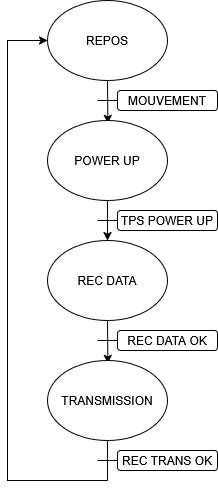
\includegraphics[width=0.2\textwidth]{Images/WP1_2/Tache_4/Automate_N1.png}
    \caption{Automate de gestion du module - version 1}
\end{figure}

Nous avons aussi décidé d'ajouter un module de capture de la tension de la batterie, afin de pouvoir surveiller la tension de la batterie, 
pouvoir faire des statistiques et aussi de permettre à l'utilisateur de savoir quand il faut changer la batterie, ou de faire des 
prévisions sur l'autonomie restante.
\\

Celui-ci repose sur le même principe que la photorésistance, c'est à dire un montage de diviseur de tension, qui nous permet de 
convertir la tension de la batterie en une tension mesurable par l'ESP32. Nous choisissons une forte valeur de résistance pour moins 
consommer.
\\

\begin{figure}[H]
    \centering
    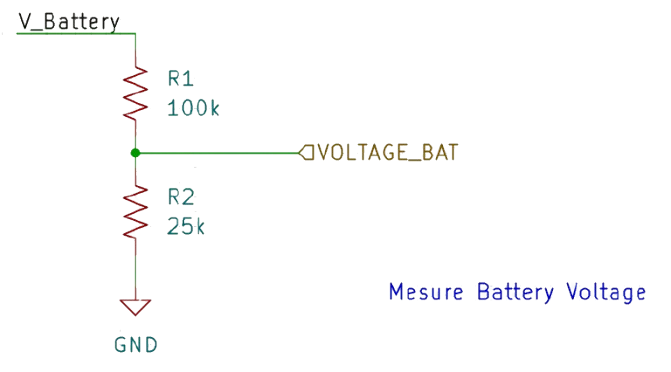
\includegraphics[width=0.8\textwidth]{Images/WP1_2/Tache_4/MesureBAT.png}
    \caption{Schéma du montage de diviseur de tension pour la mesure de la tension de la batterie}
\end{figure}

La deuxième résistance permet de connaître la division de ce montage, nous avons décidé de diviser par 4 notre système, car la tension de la 
batterie sera proche de 12V, celle-ci ne peut pas être directement mesurée par l'ESP32 qui ne supporte que 5V. En divisant par 4 nous nous
assurons que la tension mesurée ne dépassera pas 3V, ce qui est sécuritaire pour l'ESP32.
\\

\[
    V_{out} = \frac{R2}{R1 + R2} \times V_{in}
\]

La lecture de notre tension se fait grâce à un ADC ( Analog to Digital Converter ), qui convertit la tension analogique en une valeur numérique 
que l'ESP32 peut traiter. 
\\

Voici la version finale que nous avons mise en place pour la finalité de notre projet : 

\begin{figure}[H]
    \centering
    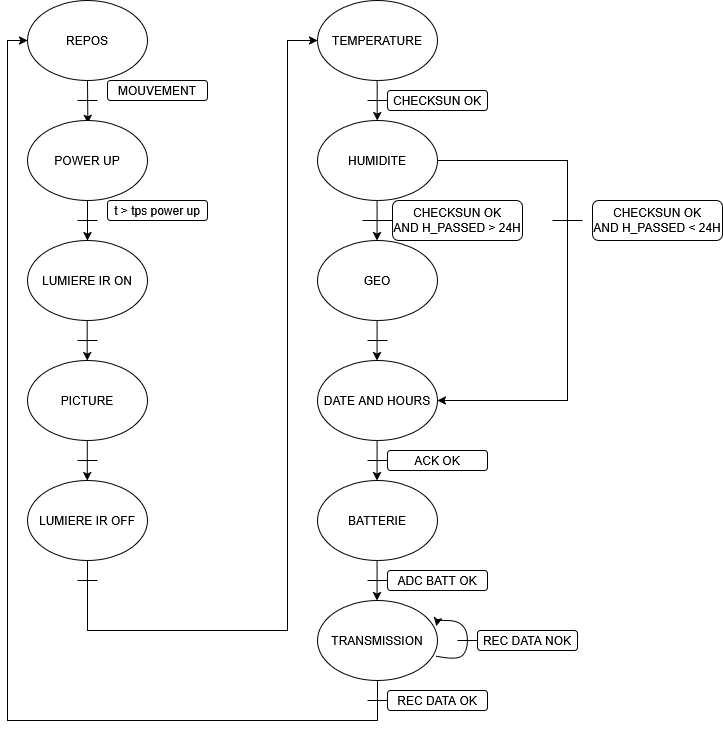
\includegraphics[width=0.8\textwidth]{Images/WP1_2/Tache_4/automate_final.png}
    \caption{Automate de gestion du module - version finale}
\end{figure}

La description de cet automate n'est pas finie, car il nous manque les étapes de transition, mais dans l'ensemble nous avons 
la structure de base de notre automate, qui nous permettra de gérer les différentes étapes de notre projet. 
\\

Nous observons toutes les étapes en commençant par le réveil de notre système par un mouvement. Une phase de réveil est nécessaire 
pour que le système puisse s'initialiser. Tout de suite après, nous allumons la couronne de LED, puis prenons une photo, puis réalisons l'extinction de celle-ci.
Nous avons effectué cela car notre couronne est en 12V et celle-ci consomme énormément d'énergie. À la suite de la prise de photo, nous prenons nos données de température, d'humidité, 
et de localisation et d'horodatage, puis nous éteignons le GPS pour économiser de l'énergie, et ensuite nous transmettons les données collectées.
Le GPS est activé seulement une fois toutes les 24h pour économiser l'énergie nécessaire à la recherche.
\\

\subsubsection{Tâche 5 : Gestion de l'alimentation du module}

\subsubsection*{Rappel des objectifs}

Dans cette tâche, j'ai dû réaliser un bilan des meilleurs moyens d'alimenter les modules afin de moins consommer d'énergie et 
d'avoir une autonomie plus longue. En effet notre projet est destiné à être utilisé dans des zones isolées, et il est donc 
essentiel d'avoir une autonomie suffisante pour que le système puisse fonctionner pendant une longue période sans besoin 
de maintenance fréquente.
\\

\subsubsection*{Solution envisagée}

Pour la première étape il faut pouvoir mettre en veille les modules afin de pouvoir mieux gérer l'énergie : 
Commençons par l'ESP32, celui-ci offre plusieurs modes de veille qui permettent de réduire considérablement la consommation d'énergie 
lorsque le système n'est pas actif.
\\

Voici les différents modes de veille disponibles pour l'ESP32 :

\begin{table}[H]
    \centering
    \small
    \renewcommand{\arraystretch}{1.25}
    \setlength{\tabcolsep}{4pt}
    \begin{tabularx}{\textwidth}{|>{\raggedright\arraybackslash}p{2.2cm}|>{\raggedright\arraybackslash}p{3cm}|>{\raggedright\arraybackslash}X|>{\raggedright\arraybackslash}X|>{\raggedright\arraybackslash}p{3.2cm}|}
        \hline
        \textbf{Mode} & \textbf{Consommation typique} & \textbf{Ce qui est éteint} & \textbf{Ce qui reste actif} & \textbf{Comment se réveiller} \\
        \hline
        \textbf{Actif} & \ensuremath{\sim 40\,\mathrm{mA} - 240\,\mathrm{mA}} & Rien & Tout & - \\
        \hline
        \textbf{Modem Sleep} & \ensuremath{\sim 20\,\mathrm{mA}} & WiFi / BT / Radio & CPU, mémoire, périphériques & Timer, interruption \\
        \hline
        \textbf{Light Sleep} & \ensuremath{\sim 0{,}8\,\mathrm{mA}} & CPU, PLL, radio & RTC, mémoire RTC, ULP co-processor & Timer, interruption (GPIO, UART, etc.) \\
        \hline
        \textbf{Deep Sleep} & \ensuremath{\sim 10\,\mu\mathrm{A} - 150\,\mu\mathrm{A}} & Presque tout : CPU, WiFi, BT, RAM principale & RTC, mémoire RTC lente (8 KB), ULP co-processor & Timer, épingles RTC, GPIO, touch \\
        \hline
        \textbf{Hibernation} & \ensuremath{\sim 2{,}5\,\mu\mathrm{A} - 5\,\mu\mathrm{A}} & Tout, même le RTC est ralenti & Mémoire RTC lente (8 KB) & Timer RTC externe uniquement \\
        \hline
    \end{tabularx}
    \caption{Principaux modes de veille de l'ESP32}
    \label{tab:esp32_sleep_modes}
\end{table}

Dans notre projet nous avons pour objectif de consommer le moins possible mais aussi de pouvoir utiliser le module RTC pour la mémoire de la localisation et l'horodatage,
ce qui nous a permis de choisir le mode de veille "Deep Sleep", qui offre une consommation très faible tout en permettant au RTC de continuer à fonctionner, 
ce qui est essentiel pour notre projet.
\\

Plusieurs autres méthodes sont envisagées pour pouvoir réduire la consommation d'énergie, comme l'arrêt de différents périphériques de ce microcontrôleur, ou encore la mise 
en place de pull-down sur les GPIO pour éviter les fuites de courant, mais après la phase de test nous nous sommes rendu compte que, à part le Wi-Fi et le Bluetooth,
le reste est négligeable en termes de consommation.
\\

Ce qui a le plus d'impact sur la consommation, c'est surtout de réduire la fréquence d'utilisation du processeur du microcontrôleur, mais cela aura un impact 
sur le temps de traitement et la rapidité d'exécution de notre code.

\subsubsection*{Tests et Validation}

Nous pouvons observer tout d'abord, afin d'avoir une idée de la consommation de base, un code vierge injecté dans l'ESP32 : 

\begin{figure}[H]
    \centering
    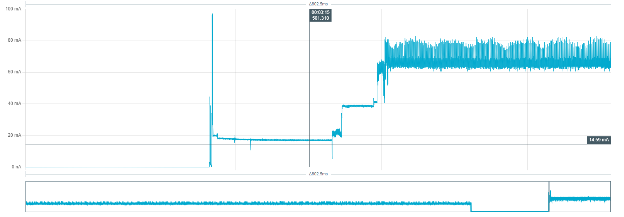
\includegraphics[width=0.8\textwidth]{Images/WP1_2/Tache_5/Code_Vierge.png}
    \caption{Consommation de base de l'ESP32 avec un code vierge}
\end{figure}

Celui-ci montre une consommation de 80mA environ.
\\

Passons maintenant à la réduction de la fréquence de notre microcontrôleur : 

\begin{figure}[H]
    \centering
    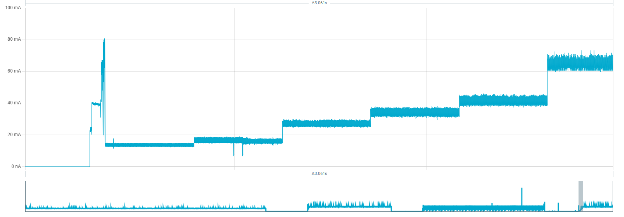
\includegraphics[width=0.8\textwidth]{Images/WP1_2/Tache_5/Frequence.png}
    \caption{Consommation de l'ESP32 en fonction de la fréquence du processeur}
\end{figure}

Dans ce graphe nous observons différents paliers qui correspondent à différentes fréquences du processeur, en commençant par 
20, 40, 80, 160 et 240 MHz. Déjà nous avons une nette différence entre toutes ces fréquences.
\\

Continuons avec le mode de veille : les modes \texttt{Deep} : 

\begin{figure}[H]
    \centering
    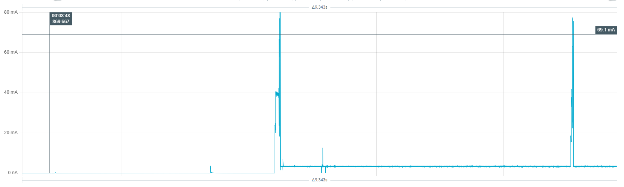
\includegraphics[width=0.8\textwidth]{Images/WP1_2/Tache_5/Deep.png}
    \caption{Consommation de l'ESP32 en fonction du mode de veille}
\end{figure}

La consommation en mode Deep Sleep est de l'ordre de 5mA en moyenne, ce qui sera un avantage pour notre projet.
\\

Pour aller plus loin dans nos tests nous avons testé la consommation en mode Deep Sleep, avec réveil par une simulation de mouvement, donc en envoyant 
un signal sur un GPIO ( simulant le PIR ).

\begin{figure}[H]
    \centering
    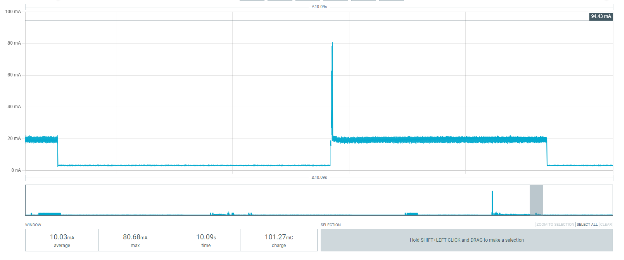
\includegraphics[width=0.8\textwidth]{Images/WP1_2/Tache_5/Deep_PIR.png}
    \caption{Consommation de l'ESP32 en mode Deep Sleep avec réveil par signal GPIO (simulant le PIR)}
\end{figure}

Celui-ci montre un système concluant, avec une faible consommation. Mais nous observons dans tous nos graphes un problème majeur, c'est un pic 
au démarrage, celui-ci correspond à l'initialisation de tous les périphériques de base de l'ESP32.

Voici un exemple de code utilisé pour le test du mode de veille :
\begin{lstlisting}[style=CStyle, caption={Exemple de code pour le test du mode de veille}, label={lst:deep_sleep_exemple}]
#define LED_PIN 2
#define WAKE_PIN 33

void actionAuReveil() 
{
  // Se declenche UNE SEULE FOIS par front montant
  digitalWrite(LED_PIN, HIGH);
  delay(150);
  digitalWrite(LED_PIN, LOW);
  delay(150);
}

void setup() 
{
    setCpuFrequencyMhz(80);

    pinMode(LED_PIN, OUTPUT);
    pinMode(WAKE_PIN, INPUT_PULLDOWN);

    digitalWrite(LED_PIN, LOW);

    // Cause de reveil 
    esp_sleep_wakeup_cause_t cause = esp_sleep_get_wakeup_cause();

    if (cause == ESP_SLEEP_WAKEUP_EXT0) 
    {
        // Execute l'action UNE seule fois
        actionAuReveil();
        while (digitalRead(WAKE_PIN) == HIGH) {}
    }

    // Rearmer le front montant UNIQUEMENT quand la pin est basse
    esp_sleep_enable_ext0_wakeup((gpio_num_t)WAKE_PIN, 1);

    esp_deep_sleep_start();
}

void loop() {}

\end{lstlisting}

\subsubsection{Tâche 6 : Intégration des modules}

\subsubsection*{Rappel des objectifs}

Dans cette phase nous avons eu pour objectif d'assembler nos modules de tout le WP1, celui-ci correspond à notre premier prototype de notre système.
Il s'agit de rassembler le travail effectué par chacun, notamment sur la partie de récupération d'images et de métadonnées, 
la partie de stockage sur la carte SD, la partie de localisation et d'horodatage, et la partie transmission.
\\

\subsubsection*{Solution envisagée}

Pour cela, nous avions décidé que chacun d'entre nous effectuerait une bibliothèque pour que je puisse simplement appeler les fonctions telles que 
l'automate défini précédemment. 
\\

Donc pour résumer la partie de notre système, le WP possède un total de 7 bibliothèques, qui sont :
\begin{itemize}
    \item CAM.hpp : bibliothèque de gestion de la caméra, qui permet de prendre des photos 
    \item GPS.hpp : bibliothèque de gestion du module GPS, qui permet de récupérer la localisation et l'horodatage
    \item RTC.hpp : bibliothèque de gestion du module RTC, qui permet de maintenir l'heure en temps réel
    \item SD.hpp : bibliothèque de gestion de la carte SD, qui permet de stocker les données collectées
    \item SENDWIFI.hpp : bibliothèque de gestion de la transmission des données en Wi-Fi
    \item BAT.hpp : bibliothèque de récupération de la tension de la batterie
    \item CONFIG.h : fichier de configuration du projet, qui contient les différentes constantes et paramètres du projet
    \\
\end{itemize}

Le code étant conséquent, il sera disponible en annexe.

\subsubsection*{Tests et Validation}

Au départ pour notre système nous avions comme objectif de faire 10 photographies et de les sauvegarder sur la carte SD, 
avec les métadonnées de localisation et d'horodatage, ainsi que les données de température et d'humidité.
\\

\begin{figure}[H]
    \centering
    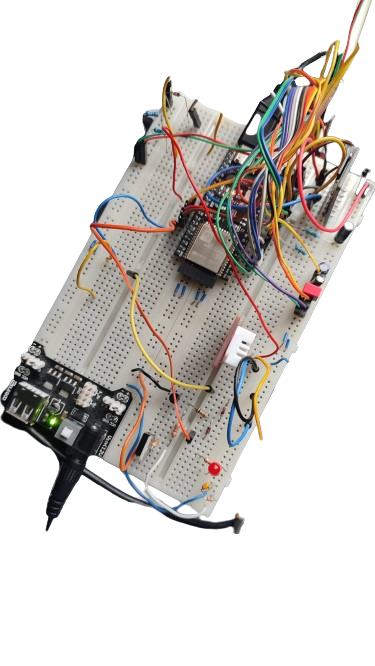
\includegraphics[width=0.4\textwidth]{Images/WP1_2/Tache_6/Proto.png}
    \caption{Prototype du système avec tous les modules intégrés}
\end{figure}

\begin{figure}[H]
    \centering
    \begin{minipage}[t]{0.45\textwidth}
        \centering
        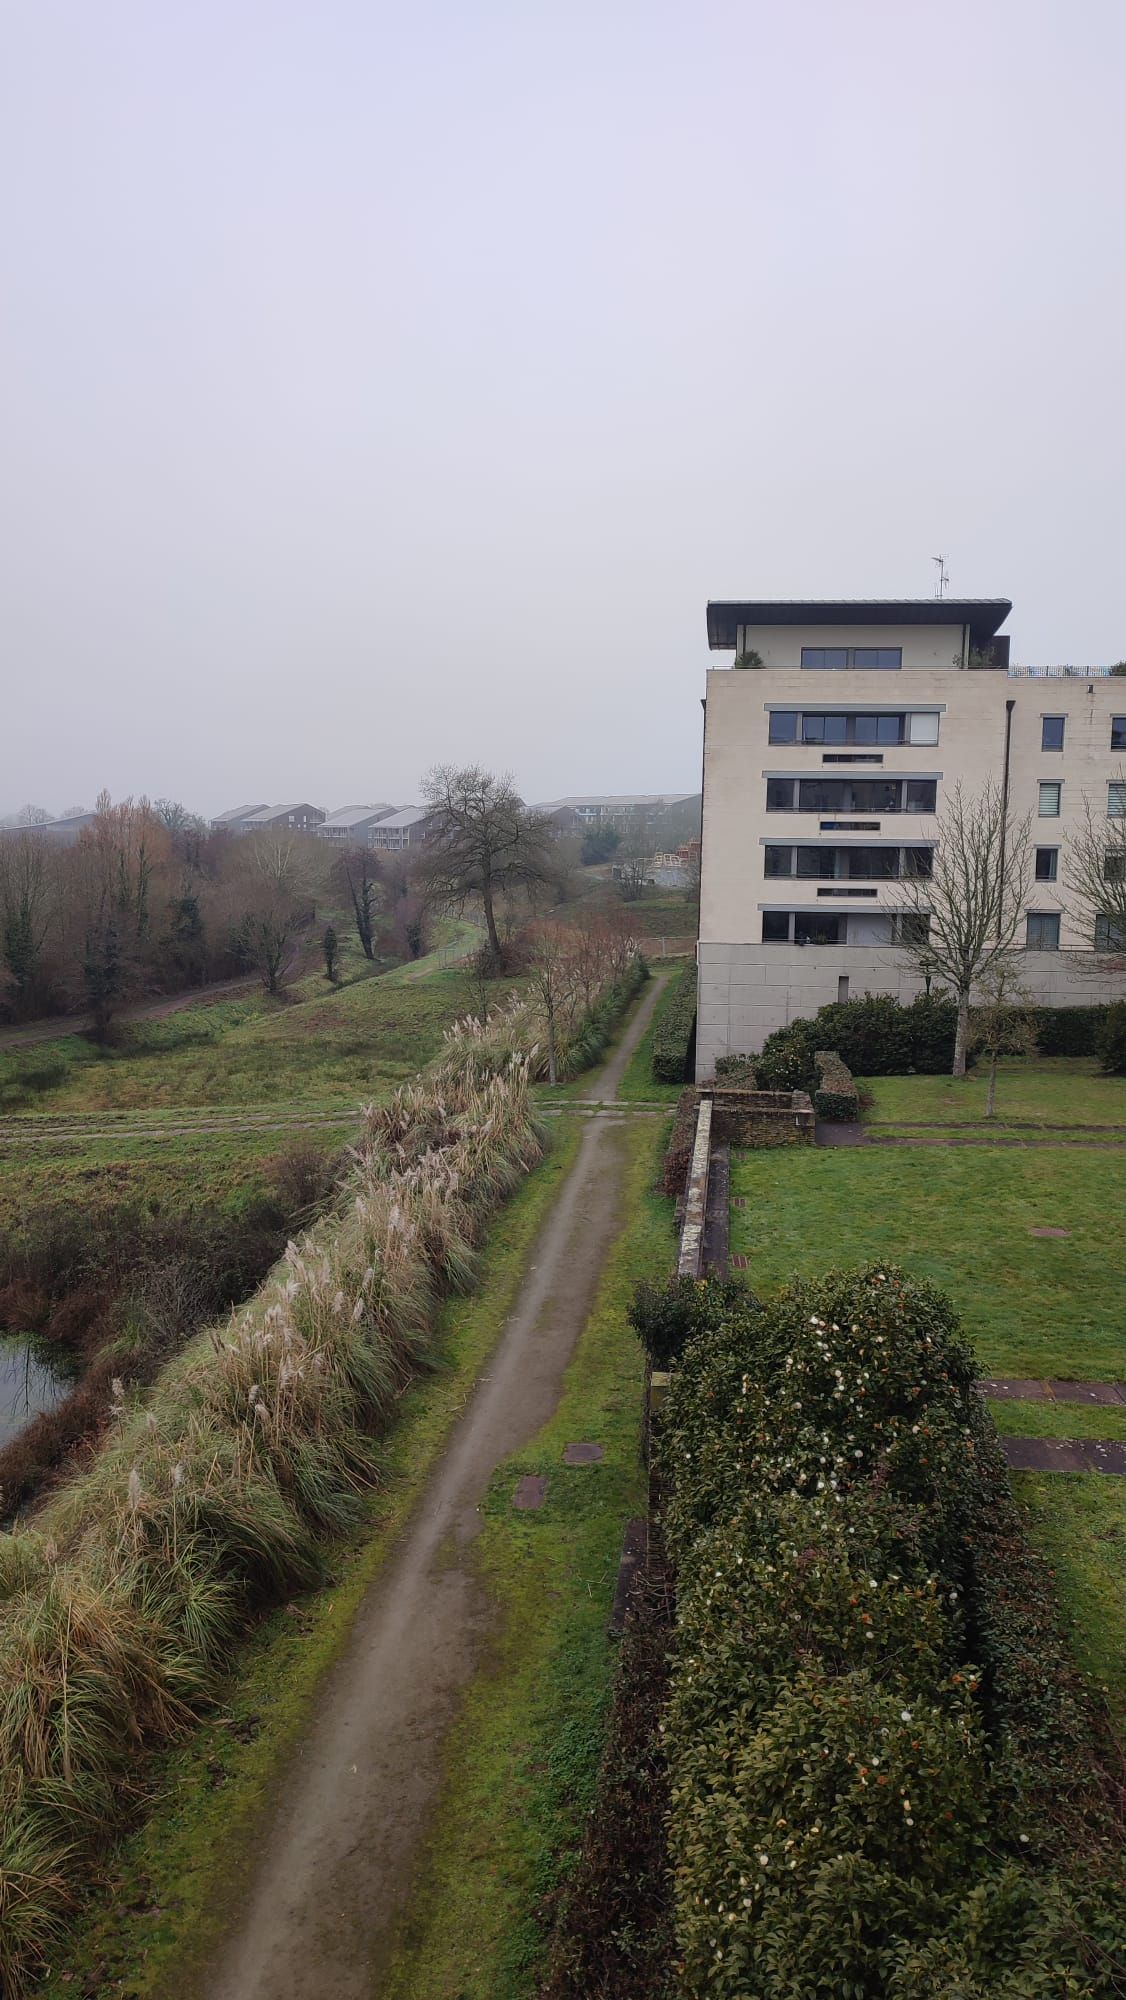
\includegraphics[width=\linewidth]{Images/WP1_2/Tache_6/Exterieur_telephone.jpeg}
        \par\small Photographie Téléphone
    \end{minipage}
    \hfill
    \begin{minipage}[t]{0.45\textwidth}
        \centering
        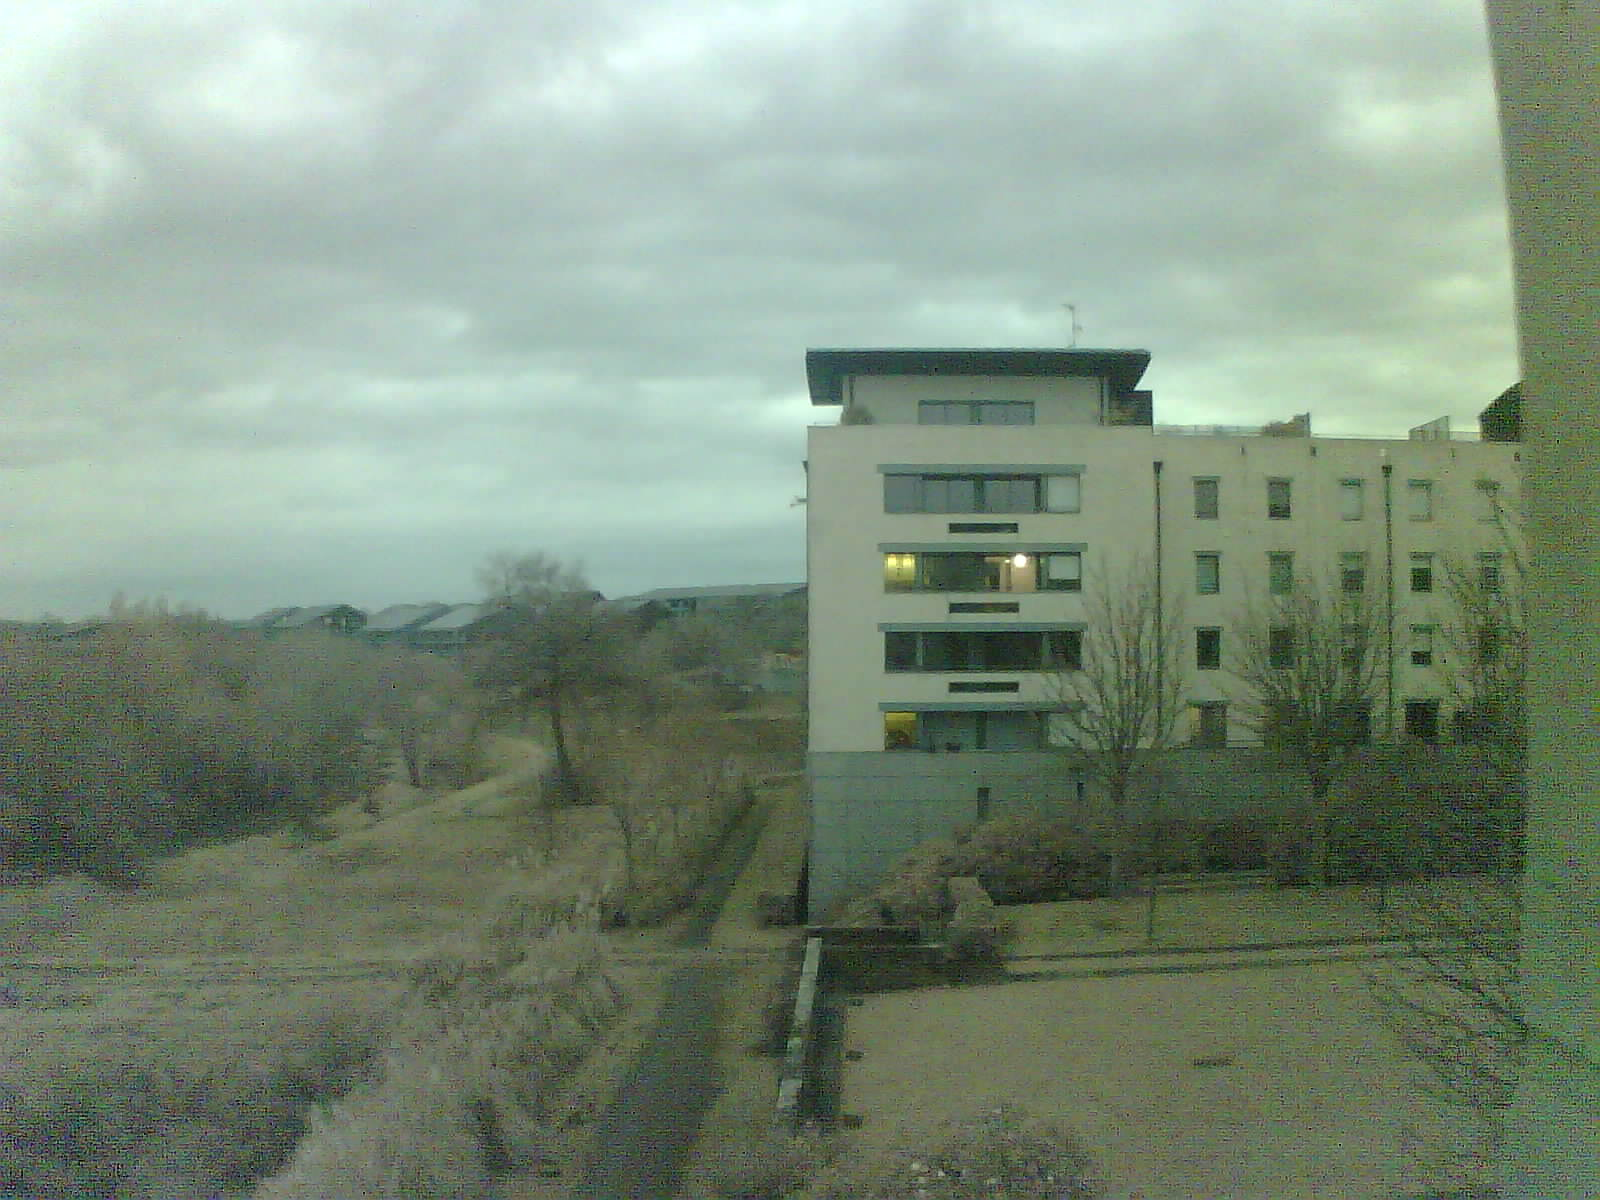
\includegraphics[width=\linewidth]{Images/WP1_2/Tache_6/Exterieur.png}
        \par\small Photographie Caméra
    \end{minipage}
    \caption{Différence entre la photographie de notre Caméra et de notre Téléphone}
\end{figure}

\begin{figure}[H]
    \centering
    \begin{minipage}[t]{0.45\textwidth}
        \centering
        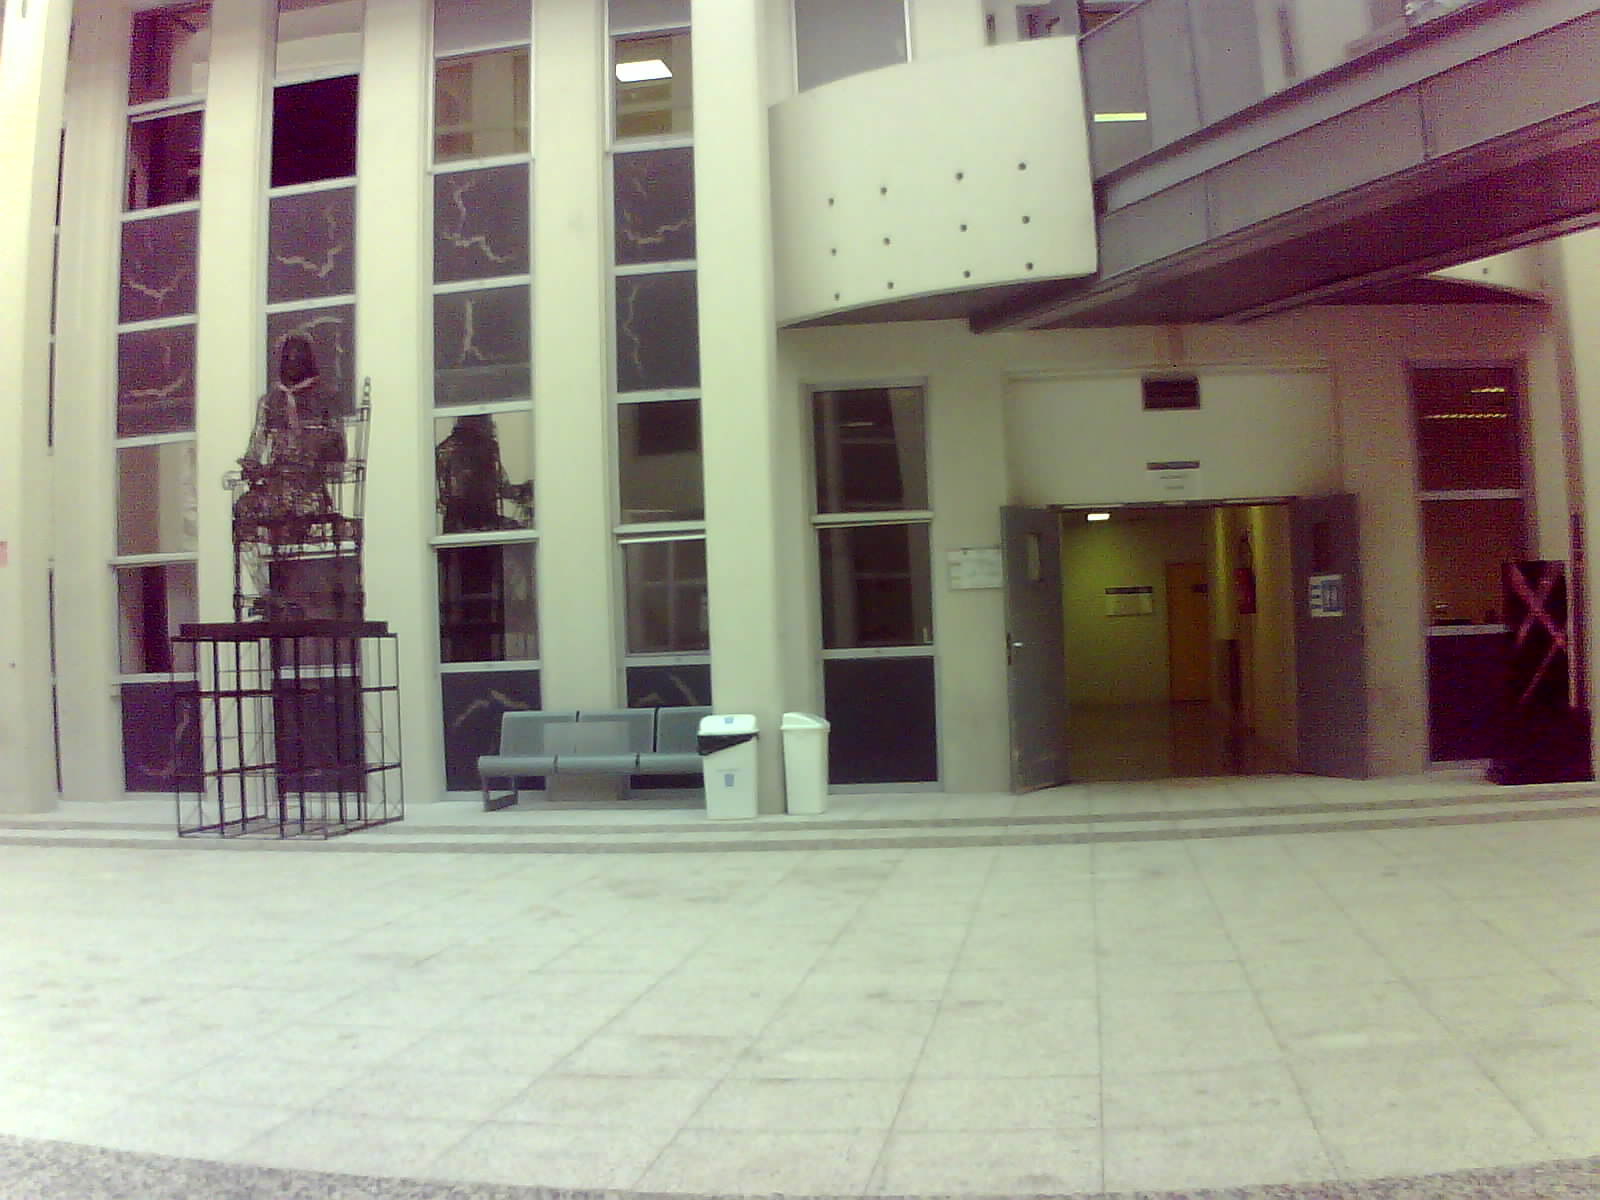
\includegraphics[width=\linewidth]{Images/WP1_2/Tache_6/Interieur.png}
        \par\small Photographie intérieure
    \end{minipage}
    \hfill
    \begin{minipage}[t]{0.45\textwidth}
        \centering
        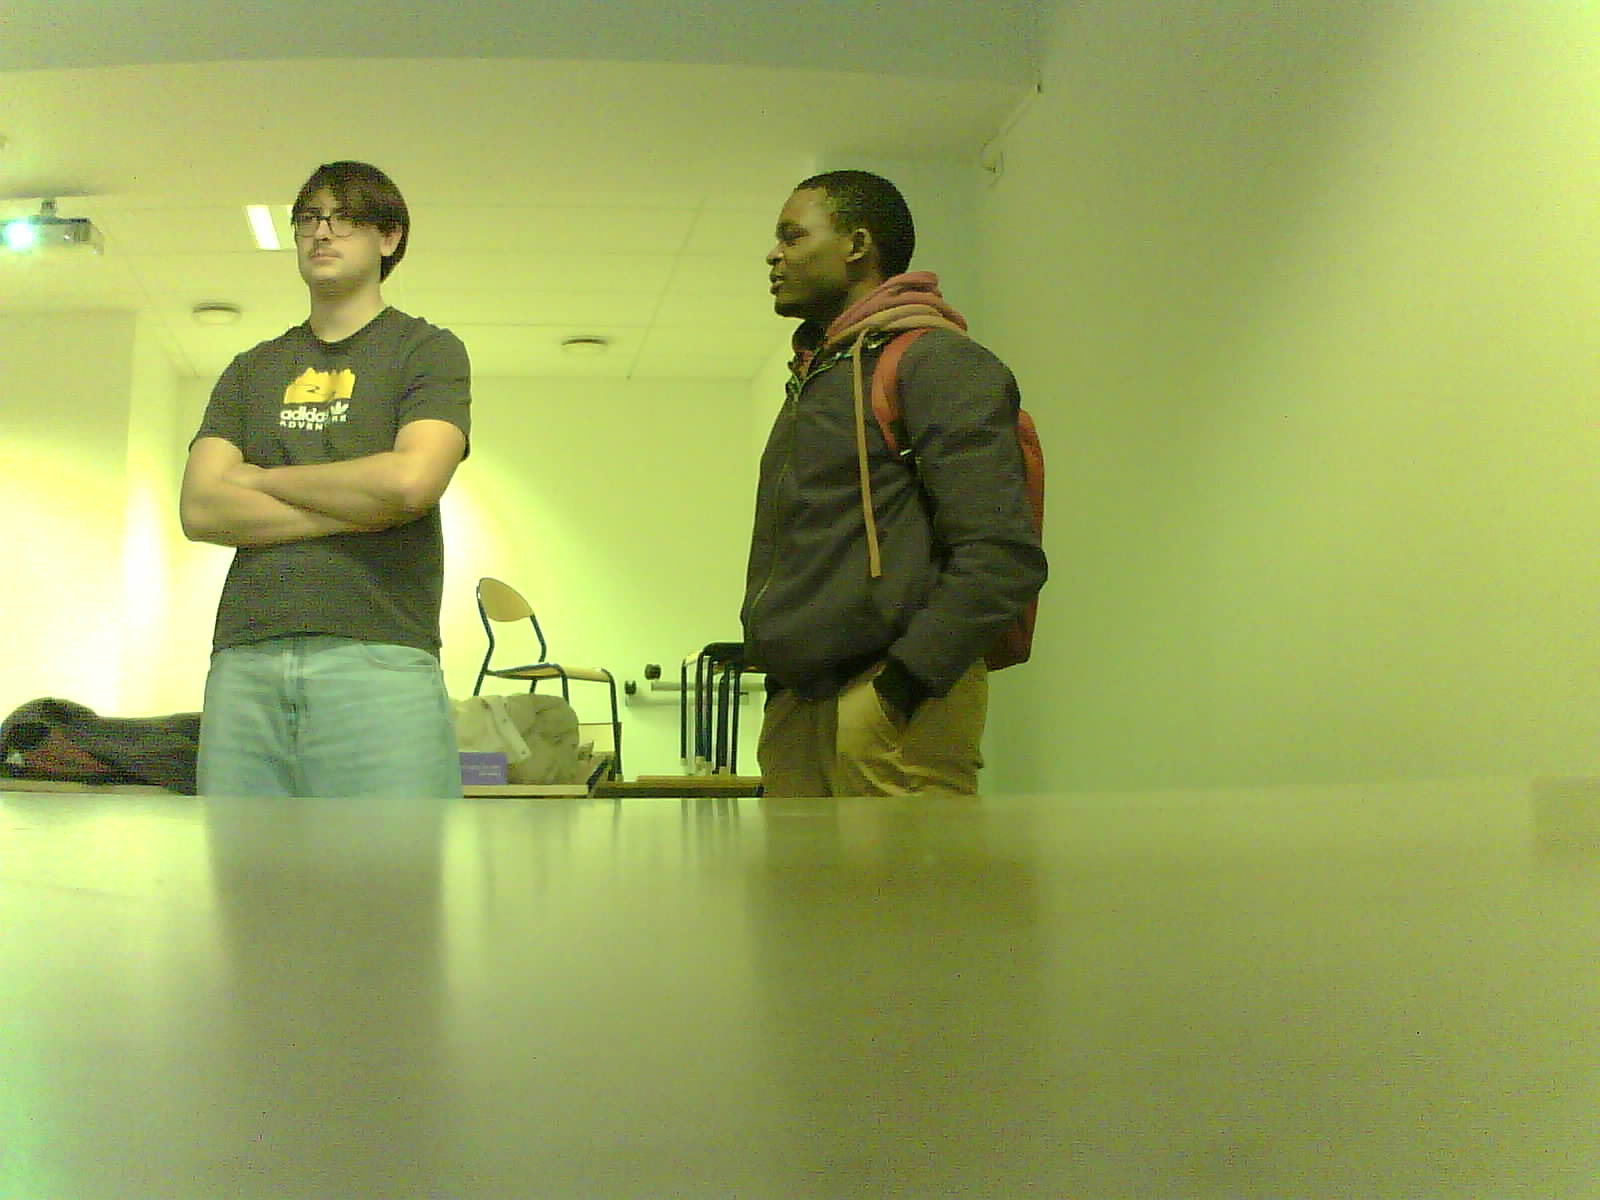
\includegraphics[width=\linewidth]{Images/WP1_2/Tache_6/Humain.png}
        \par\small Photographie Humain
    \end{minipage}
    \caption{Autre section de notre architecture}
\end{figure}

Cependant notre équipe a été assez performante, et à peine la réalisation de ce prototype terminée, nous avons pu faire des tests 
de transmission en Wi-Fi et de réception sur le serveur de stockage distant. 
\\

Un problème majeur est survenu lors de nos phases de test, c'était tout simplement la résolution de nos photos. De base la bibliothèque de 
la caméra nous permettait de choisir l'emplacement du buffer de l'image, mais malheureusement notre ESP32 personnel n'était pas assez puissant 
et nous étions obligés de stocker l'image dans la DRAM ( stockage principal de l'ESP32 ), qui est limitée en termes de capacité, et qui ne nous 
permettait pas de stocker des images de haute résolution. De plus nous ne pouvions pas utiliser la carte SD pour stocker le buffer car le moyen
de récupération de l'image ( Méthode DMA ( Direct Memory Access ) ) n'est pas compatible avec la carte SD.
\\

Pour faire face à ce problème nous avons donc décidé de regarder la bibliothèque en détail, et nous avons trouvé une solution adaptée à notre problème, qui a 
été de prendre un ESP32 avec une PSRAM. Une PSRAM ( pseudo-static RAM ) est une mémoire externe qui peut être utilisée pour stocker des données, 
et qui offre une capacité plus grande que la DRAM interne de l'ESP32 ; celle-ci est directement connectée à un périphérique de l'ESP32 ( I2S ), 
ce qui nous a permis de stocker des images de haute résolution sans problème de stockage.
\\

\begin{figure}[H]
    \centering
    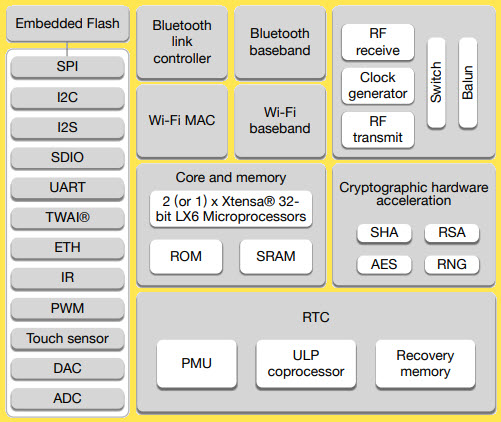
\includegraphics[width=0.6\textwidth]{Images/WP1_2/Tache_6/ESP32-Block-Diagram.jpg}
    \caption{Schéma de l'architecture du système avec l'ESP32 et la PSRAM pour le stockage des images}
\end{figure}

Donc nous sommes partis sur un modèle plus haut de gamme de l'ESP32, qui est l'ESP32-WROVER, qui intègre une PSRAM de 8MB. Une amélioration ne 
vient pas toute seule, ce modèle possède aussi plus de pins GPIO que notre ancien modèle qui arrivait à saturation.
\\

\subsubsection{Tâche 7 : Développement d'une architecture électrique}

\subsubsection*{Rappel des objectifs}

Dans cette section il s'agit d'effectuer une étude de notre schéma réalisé grâce au prototype, car celui-ci étant concluant, il nous permet 
de construire notre schéma électrique, qui nous permettra de construire potentiellement un PCB à l'avenir, ou de faire une meilleure gestion 
de l'alimentation et de la consommation de notre système.
\\

\subsubsection*{Solution envisagée}

Dans un premier temps, nous recopions juste notre système grâce au logiciel de CAO, \textbf{Kicad}. Pour que cela soit plus parlant et mieux en 
terme de gestion de projet, nous mettons des blocs pour que chaque partie soit clairement identifiée.
\\

\begin{figure}[H]
    \centering
    
\includegraphics[width=1\textwidth]{Images/WP1_2/Tache_7/Main.pdf}
    \caption{Schéma électrique global du système réalisé avec Kicad}
\end{figure}

Celui-ci montre notre WP1 dans son ensemble avec les différents modules. Commençons par notre partie principale qui est notre microcontrôleur.
Celle-ci montre notre microcontrôleur avec toutes les pins utilisables. Nous ajoutons des pull-up sur les signaux I2C et des condensateurs
de découplage pour éviter les problèmes de bruit et de stabilité du système. Une diode est rajoutée, car la pin VIN est aussi la pin de sortie
de tension du câble de programmation, et cela nous permet d'éviter les problèmes de court-circuit lors de la programmation du module.
\\ 

\begin{figure}[H]
    \centering
    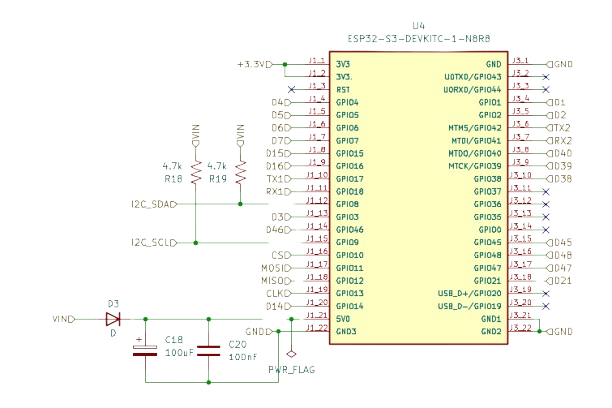
\includegraphics[width=0.8\textwidth]{Images/WP1_2/Tache_7/uc.png}
    \caption{Schéma de la partie microcontrôleur du système réalisé avec Kicad}
\end{figure}

Dans un second cas nous prenons la partie capteur, nous avons au total 3 capteurs : le GPS, le module DHT22 ( température et humidité ) et le PIR.
Nous avons décidé d'ajouter des connecteurs supplémentaires, comme un double connecteur pour notre module personnel mais aussi pour un autre module
GPS que nous avions sélectionné à commander. Nous avons aussi ajouté un transistor MOSFET pour pouvoir contrôler son alimentation.
\\

Nous avons aussi rajouté une LED de DEBUG, qui nous permettra de faire du débogage visuel de notre système, en indiquant par exemple l'état du système 
ou les différentes étapes de notre automate.
\\

Et enfin d'autres connecteurs comme deux connecteurs Grove ( pour les modules I2C ) et un connecteur pour un autre capteur de température, humidité et pression ( BME280 ) que nous avions sélectionné à commander.
Ce capteur de pression et de qualité de l'air était dans la commande initiale, mais n'est pas arrivé à temps pour les tests. Il nous permettra d'avoir des données supplémentaires sur les conditions environnementales de la zone.
\\

\begin{figure}[H]
    \centering
    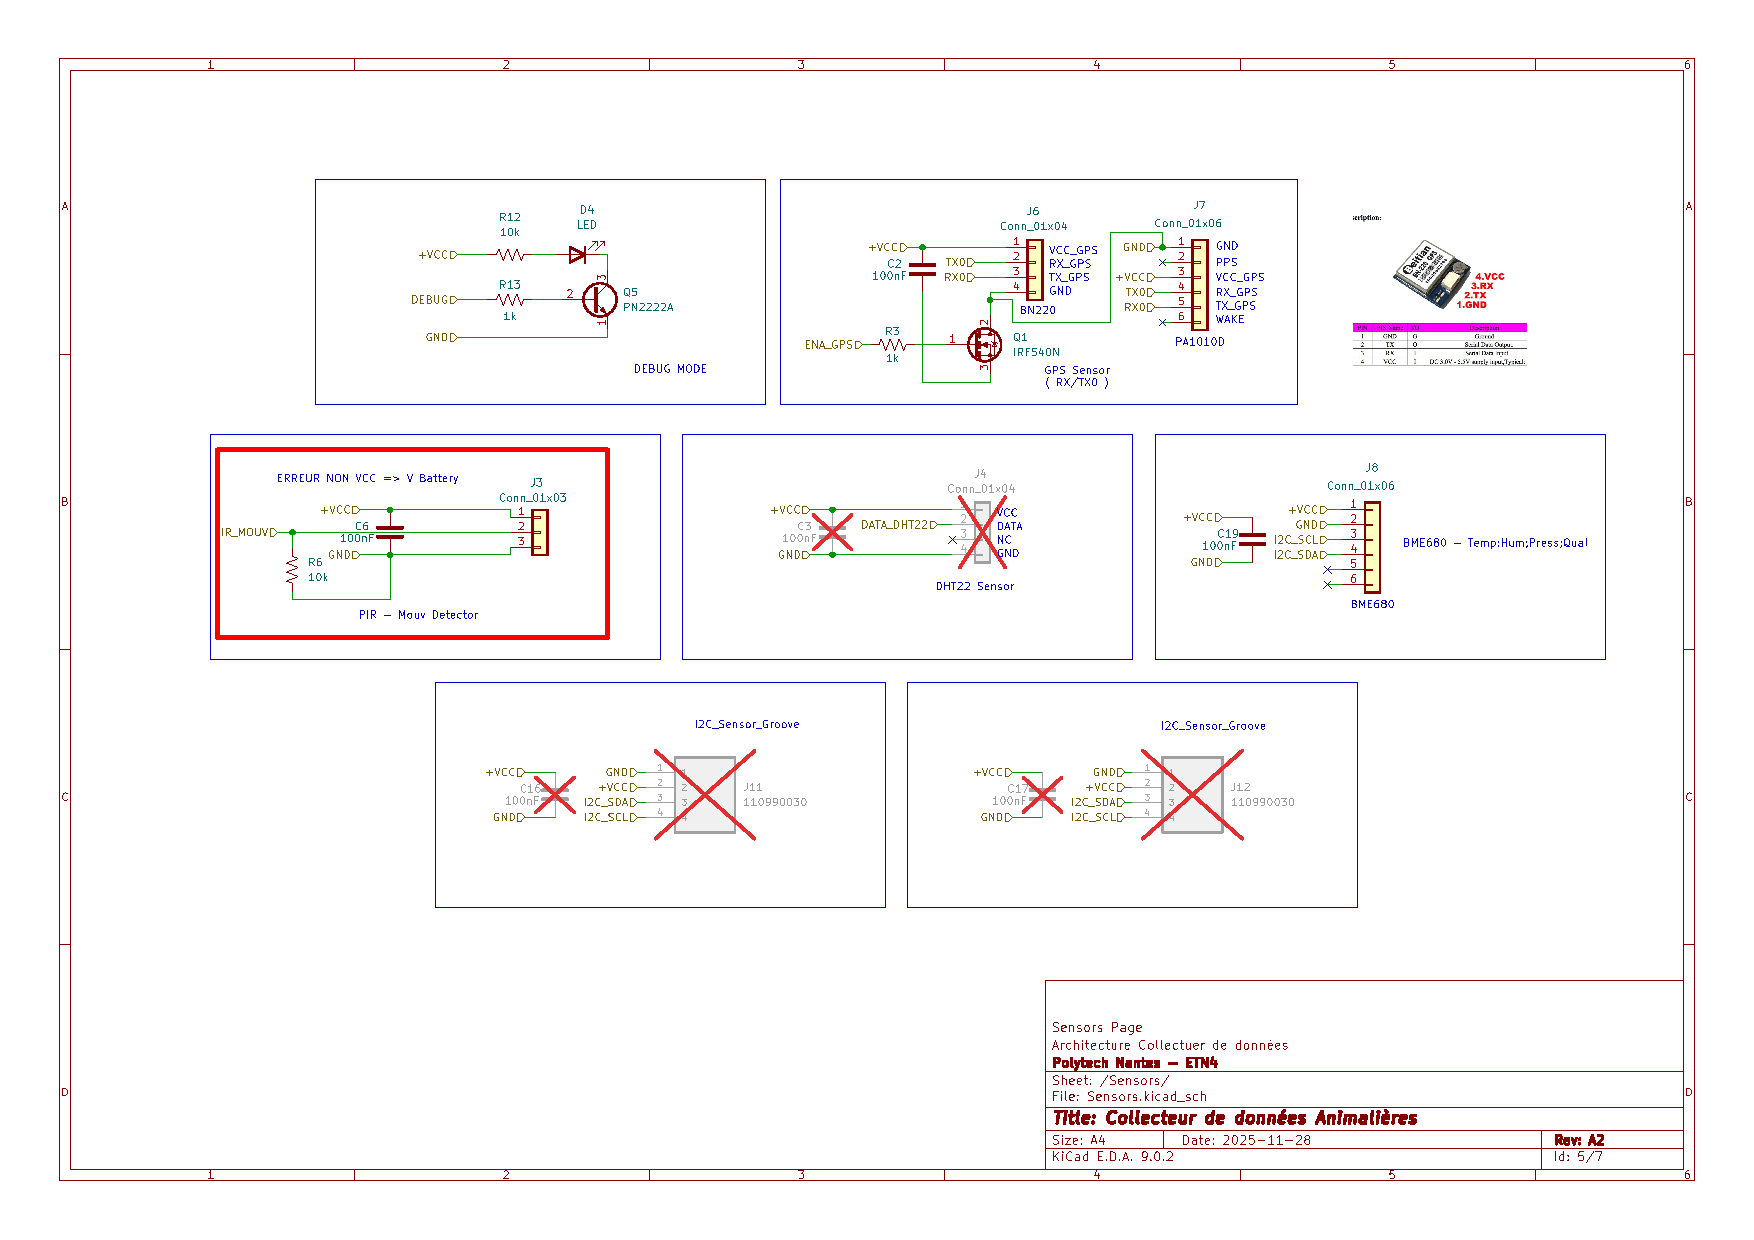
\includegraphics[width=1\textwidth]{Images/WP1_2/Tache_7/Main-Sensors.pdf}
    \caption{Schéma de la partie capteurs du système réalisé avec Kicad}
\end{figure}

Passons à la partie caméra, qui quant à elle possède un connecteur pour la caméra OV2640, mais aussi un connecteur pour la couronne de LED infrarouges. Nous avons
aussi rajouté un transistor MOSFET pour pouvoir contrôler son alimentation.

\begin{figure}[H]
    \centering
    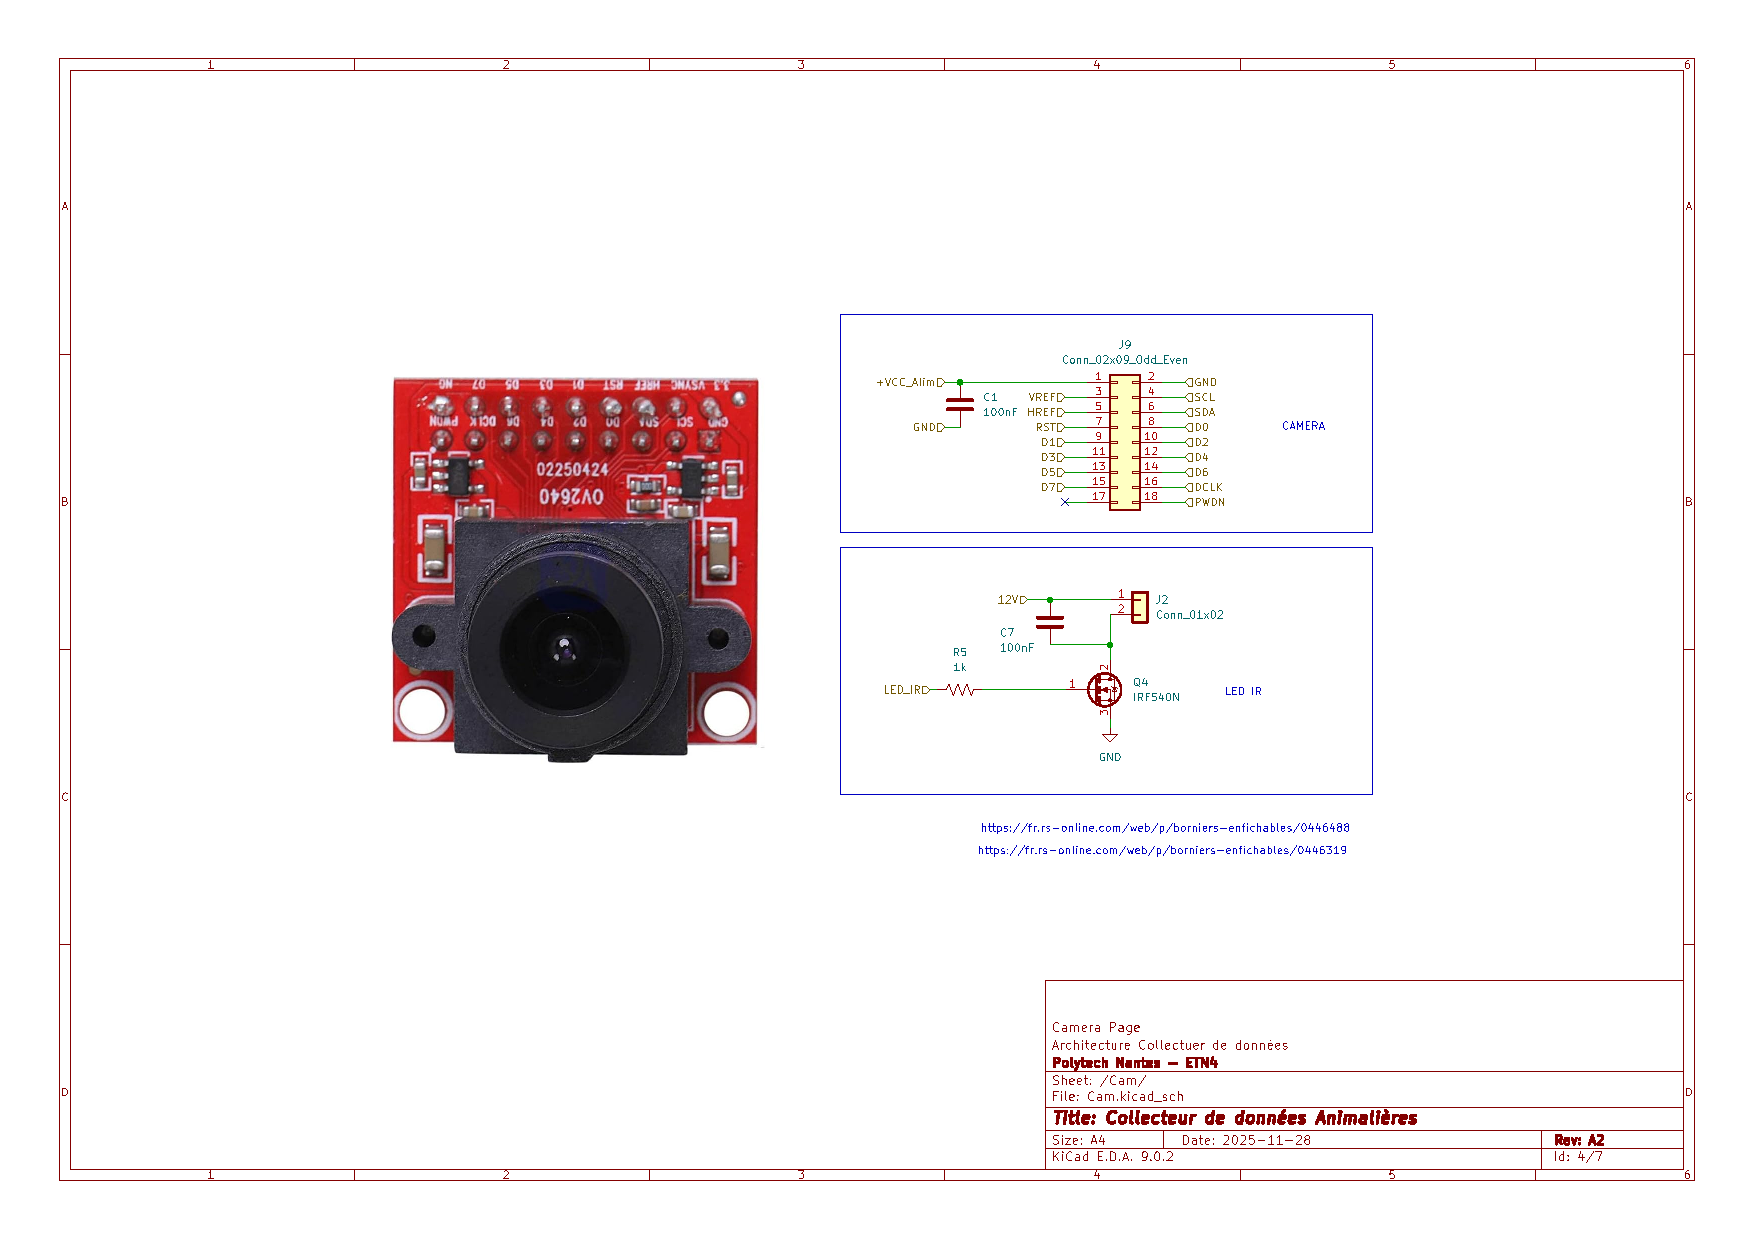
\includegraphics[width=1\textwidth]{Images/WP1_2/Tache_7/Main-Cam.pdf}
    \caption{Schéma de la partie caméra du système réalisé avec Kicad}
\end{figure}

Nous avons ensuite les connecteurs pour le module de carte SD ainsi que le futur module de carte SIM pour une transmission en 4G :

\begin{figure}[H]
    \centering
    \begin{minipage}[t]{0.48\textwidth}
        \centering
        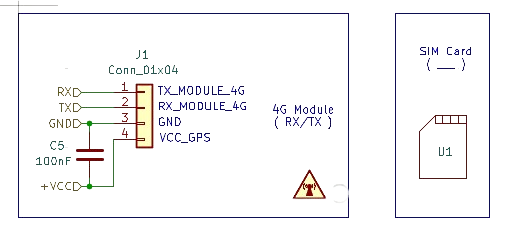
\includegraphics[width=\linewidth]{Images/WP1_2/Tache_7/4G.png}
        \par\small Connecteur pour le module 4G
    \end{minipage}
    \hfill
    \begin{minipage}[t]{0.48\textwidth}
        \centering
        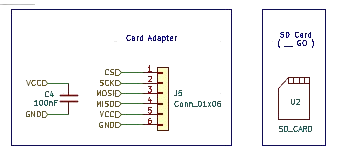
\includegraphics[width=\linewidth]{Images/WP1_2/Tache_7/SD.png}
        \par\small Connecteur pour le module de carte SD
    \end{minipage}
    \caption{Autre section de notre architecture}
\end{figure}

Enfin pour finir nous avons la partie d'alimentation, celle-ci nous a donné un peu plus de réflexion étant donné que notre système fonctionnait 
à 12V, mais que notre microcontrôleur et les autres modules fonctionnaient à 5V, nous avons donc décidé d'utiliser un régulateur de tension pour abaisser la tension de 12V à 5V.
\\

De plus il a fallu réfléchir à un moyen de pouvoir avoir une alimentation qui alimente notre ESP32 et notre PIR tout le temps afin de détecter ou non, et une autre activable 
seulement lors de la prise de photo pour alimenter la couronne de LED et la caméra, afin d'économiser de l'énergie, nous avons donc décidé d'utiliser un transistor MOSFET 
pour pouvoir contrôler l'alimentation de ces éléments.
\\

Le montage suivant est réalisé à l'aide d'un transistor MOSFET P-Channel, qui agit comme un relais en reliant le 5V du régulateur avec les différents modules.
\\

\begin{figure}[H]
    \centering
    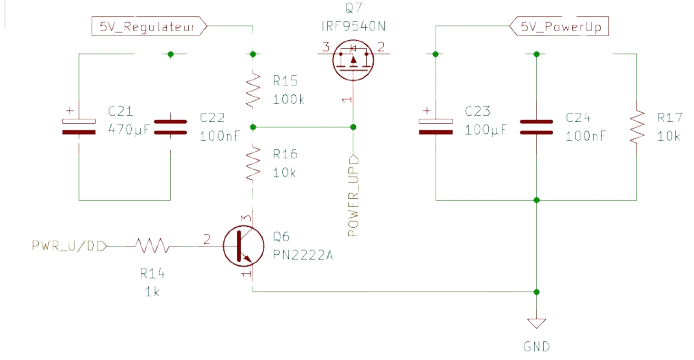
\includegraphics[width=\linewidth]{Images/WP1_2/Tache_7/Montage_PowerUp.png}
    \caption{Schéma du montage de contrôle d'alimentation avec un transistor MOSFET P-Channel}
\end{figure}

Dans ce montage si une tension à la sortie du régulateur est présente, alors le transistor est éteint et ne laisse pas passer le courant, mais lorsque la pin de contrôle du transistor est mise à LOW, 
alors le transistor s'active et laisse passer le courant, ce qui permet d'alimenter les modules connectés à la sortie du transistor. 

\begin{figure}[H]
    \centering
    \begin{minipage}[t]{0.48\textwidth}
        \centering
        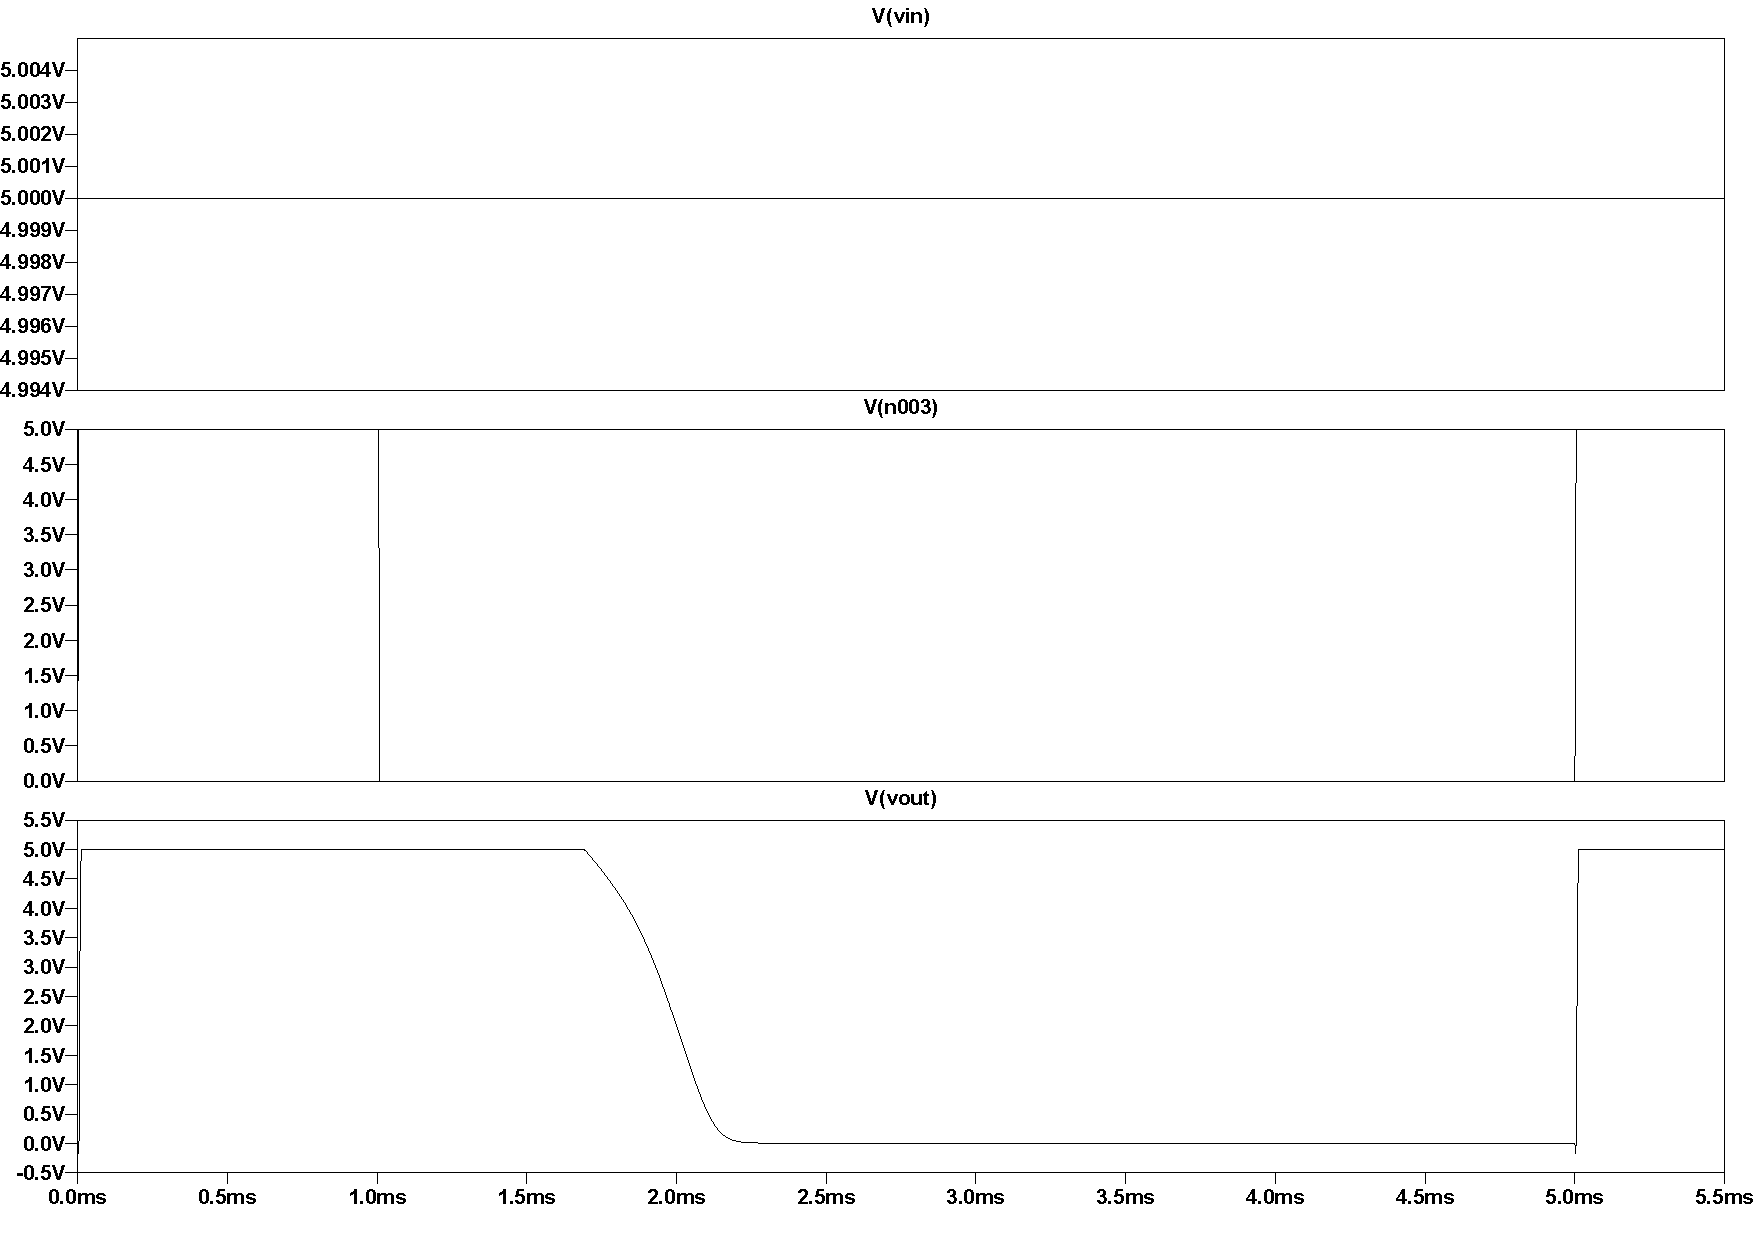
\includegraphics[width=\linewidth]{Images/WP1_2/Tache_7/Power_Up.pdf}
        \par\small Simulation du fonctionnement
    \end{minipage}
    \hfill
    \begin{minipage}[t]{0.48\textwidth}
        \centering
        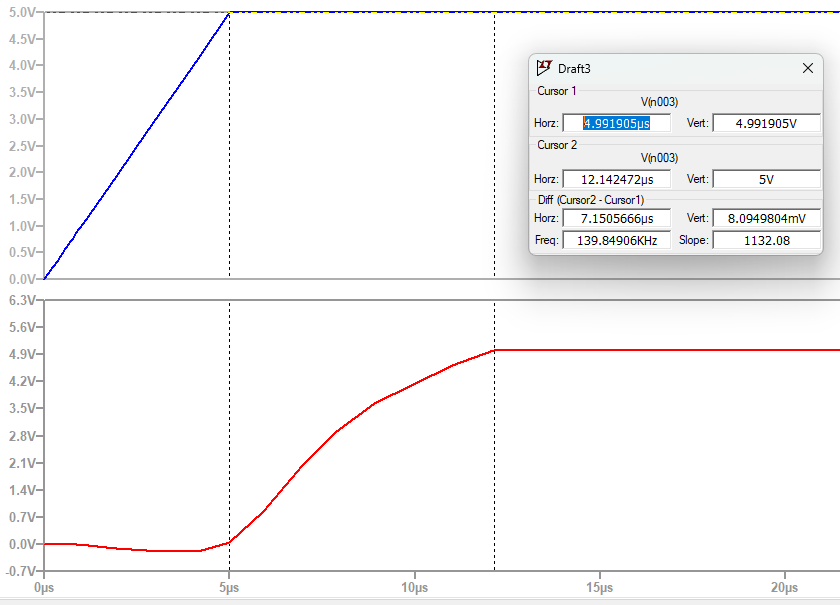
\includegraphics[width=\linewidth]{Images/WP1_2/Tache_7/delay_power_up.png}
        \par\small Simulation du délai d'activation du transistor MOSFET
    \end{minipage}
    \caption{Simulation du fonctionnement du montage de contrôle d'alimentation avec un transistor MOSFET P-Channel}
\end{figure}

Nous avons aussi observé le délai d'activation entre nos deux tensions qui est de 10us, ce qui est largement suffisant pour notre projet.
\\

Pour résumer notre schéma d'alimentation, voici un tableau récapitulatif de notre architecture d'alimentation :

\begin{table}[H]
    \centering
    \renewcommand{\arraystretch}{1.35}
    \setlength{\tabcolsep}{10pt}
    \begin{tabularx}{\textwidth}{|>{\centering\arraybackslash}p{0.28\textwidth}|>{\centering\arraybackslash}p{0.33\textwidth}|>{\centering\arraybackslash}p{0.33\textwidth}|}
        \hline
        \textbf{12V} & \textbf{5V -- Sortie Régulateur} & \textbf{5V -- Power Up} \\
        \hline
        \begin{tabular}[t]{@{}l@{}}Couronne LED\\Régulateur\end{tabular} &
        \begin{tabular}[t]{@{}l@{}}ESP32\\PIR\\Caméra (Mode Veille)\end{tabular} &
        \begin{tabular}[t]{@{}l@{}}DHT22\\Carte SD\\GPS\\4G\\DEBUG\\Autre Capteur\end{tabular} \\
        \hline
    \end{tabularx}
    \caption{Répartition des éléments selon les différentes alimentations du système}
    \label{tab:architecture_alimentation}
\end{table}

Et voici le schéma d'alimentation de notre système complet, celui-ci possède un régulateur 12V vers 5V, de chez Microchip ( Demande du client ), avec le système de power up / down, et le pont 
diviseur de notre système de mesure de la tension de la batterie :
\\

\begin{figure}[H]
    \centering
    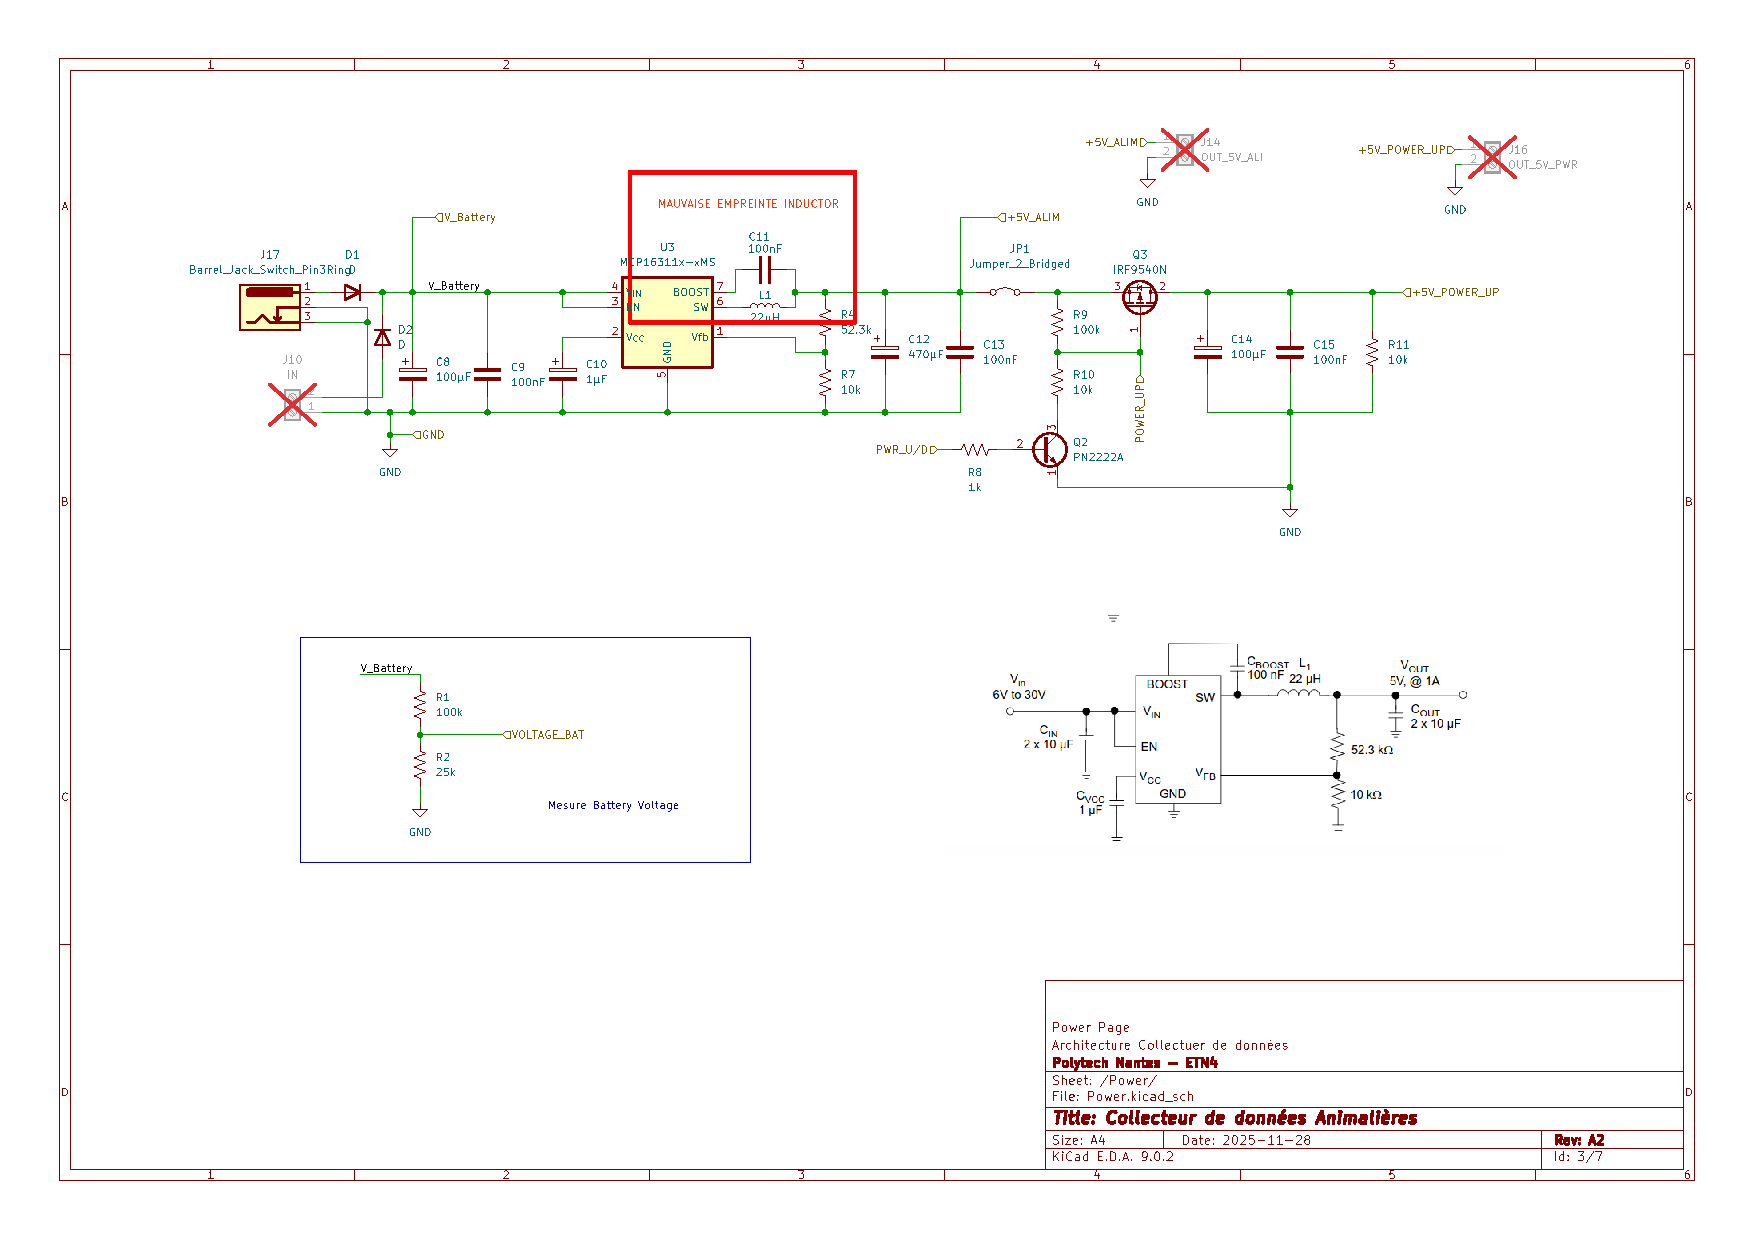
\includegraphics[width=1\textwidth]{Images/WP1_2/Tache_7/Main-Power.pdf}
    \caption{Schéma d'alimentation complet du système réalisé avec Kicad}
\end{figure}

\subsubsection{Tâche 8 : Création d'un PCB pour le module}

\subsubsection*{Rappel des objectifs}

Jusqu'à présent nous avons réalisé notre système sur une breadboard, ce qui est pratique pour les phases de test et de développement, mais qui n'est pas adapté pour une utilisation finale,
car cela peut être fragile et peu fiable. De plus cela peut engendrer des problèmes d'interférence, notamment sur la caméra qui possède des signaux de synchronisation très sensibles.
De plus notre système jusqu'à présent était alimenté via une batterie externe classique, ce qui n'est pas la finalité de notre projet.
\\

Pour aller plus loin dans notre projet, nous avons décidé de réaliser un PCB ( Printed Circuit Board ) pour notre système, ce qui nous permettra d'avoir un système plus compact, plus fiable, 
et plus facile à utiliser, sans câble volant partout. Nous continuons à utiliser le logiciel Kicad qui permet la réalisation de PCB.
\\

\subsubsection*{Solution envisagée}

Pour la première partie de conception d'un circuit imprimé nous devons attribuer une empreinte ( Footprint ) à chaque composant de notre schéma, cela permet de définir la forme et les dimensions 
de chaque composant sur le PCB, ainsi que les points de soudure pour les connexions électriques. La plupart des composants basiques comme les résistances,
inductances ou condensateurs possèdent des empreintes standard, mais pour les composants plus spécifiques comme notre microcontrôleur ou notre module de caméra, nous avons dû créer nos propres empreintes, 
en respectant les dimensions et les caractéristiques de ces composants.
\\

Pour le cas du microcontrôleur, deux connecteurs femelles pour les broches, et pour la caméra un seul connecteur 2x9 broches, qui correspond à la nappe de la caméra OV2640.
L'objectif étant de supprimer les câbles, nous avons décidé de connecter la caméra sur le PCB : 
\\

\begin{figure}[H]
    \centering
    \begin{minipage}[t]{0.35\textwidth}
        \centering
        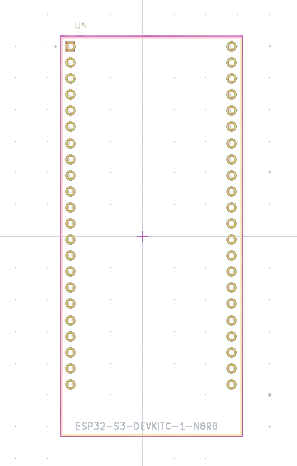
\includegraphics[width=\linewidth]{Images/WP1_2/Tache_8/FootPrint_ESP.png}
        \par\small Empreinte du microcontrôleur ESP32-WROVER
    \end{minipage}
    \hfill
    \begin{minipage}[t]{0.35\textwidth}
        \centering
        \includegraphics[width=\linewidth]{Images/WP1_2/Tache_8/FootPrint_CAM.png}
        \par\small Empreinte du module de caméra OV2640
    \end{minipage}
    \caption{Empreintes des composants sur le PCB}
\end{figure}

Pour la caméra nous choisissons d'ajouter 4 trous de fixation mécanique, deux pour la caméra, et deux autres pour la couronne de LED qui viendra par-dessus.
\\

À la suite de ça nous avons réalisé le placement des composants, celui-ci en concertation avec le WP Boîtier, qui s'occupe de la partie mécanique du projet,
afin de pouvoir faire un placement optimal des composants sur le PCB, en prenant en compte les contraintes mécaniques et d'encombrement du boîtier.
\\

À la suite nous avons réalisé le routage de la carte. Pour les règles de routage, quelque chose de basique a été réalisé : des pistes de 0.5mm pour l'alimentation 
et des pistes de 0.3mm pour les signaux. Aucune puissance n'étant réellement élevée, nous n'avons pas besoin de faire des pistes plus larges, 
et cela nous permet de gagner de la place sur le PCB.
\\

Aucun plan de masse n'a été réalisé, car notre système n'est pas sensible au bruit électromagnétique, l'isolement des pistes via des condensateurs de découplage
est suffisant pour assurer la stabilité du système, et cela nous permet de gagner de la place sur le PCB.
\\

\begin{figure}[H]
    \centering
    \begin{minipage}[t]{0.48\textwidth}
        \centering
        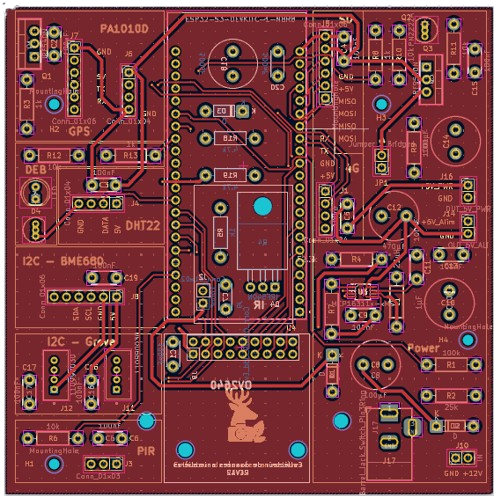
\includegraphics[width=\linewidth]{Images/WP1_2/Tache_8/TopPCB.png}
        \par\small Vue du haut du PCB
    \end{minipage}
    \hfill
    \begin{minipage}[t]{0.48\textwidth}
        \centering
        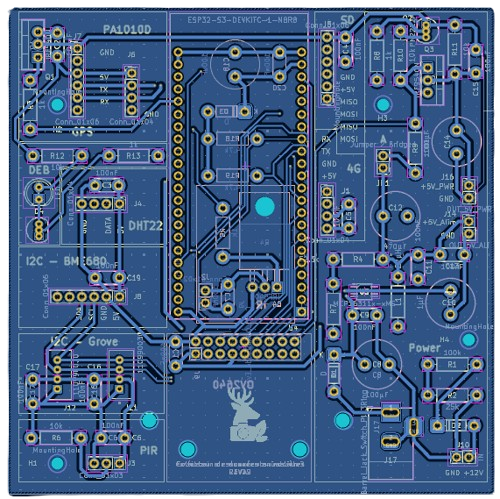
\includegraphics[width=\linewidth]{Images/WP1_2/Tache_8/BotPCB.png}
        \par\small Vue du bas du PCB
    \end{minipage}
    \caption{Rendu final du PCB réalisé avec Kicad}
\end{figure}

Voici le rendu final de notre PCB, celui-ci est réalisé en double couche, avec les composants montés des deux côtés du PCB, ce qui nous permet de gagner de la place et d'avoir un système plus compact.
\\

\begin{figure}[H]
    \centering
    \begin{minipage}[t]{0.48\textwidth}
        \centering
        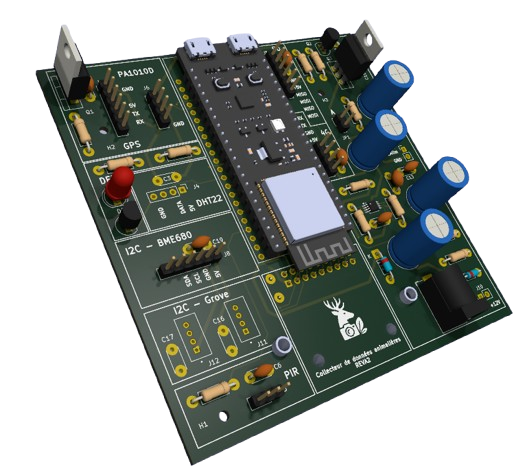
\includegraphics[width=\linewidth]{Images/WP1_2/Tache_8/3DPCB_TOP.png}
        \par\small Vue du haut du PCB
    \end{minipage}
    \hfill
    \begin{minipage}[t]{0.48\textwidth}
        \centering
        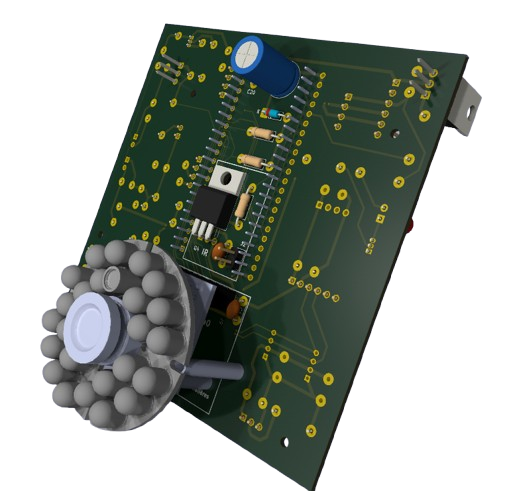
\includegraphics[width=\linewidth]{Images/WP1_2/Tache_8/3DPCB_BOT.png}
        \par\small Vue du bas du PCB
    \end{minipage}
    \caption{Rendu final 3D du PCB réalisé avec Kicad}
\end{figure}

Voici le rendu final en 3D de notre PCB, celui-ci nous permet de visualiser notre système dans son ensemble, et de vérifier que tous les composants sont correctement placés et connectés,
ainsi que de vérifier les dimensions et l'encombrement du système, ce qui est essentiel pour la suite de notre projet, notamment pour la partie mécanique du boîtier.
\\

\subsubsection*{Tests et Validation}

Après réception de notre PCB nous l'avons monté et soudé, avec le matériel que nous avions personnellement, et nous avons effectué des tests de tension.

\begin{figure}[H]
    \centering
    \begin{minipage}[t]{0.48\textwidth}
        \centering
        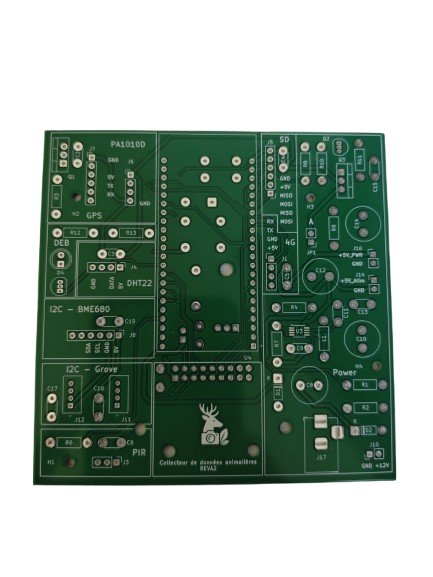
\includegraphics[width=\linewidth]{Images/WP1_2/Tache_8/PCB_TOP.png}
        \par\small Vue du haut du PCB après réception
    \end{minipage}
    \hfill
    \begin{minipage}[t]{0.48\textwidth}
        \centering
        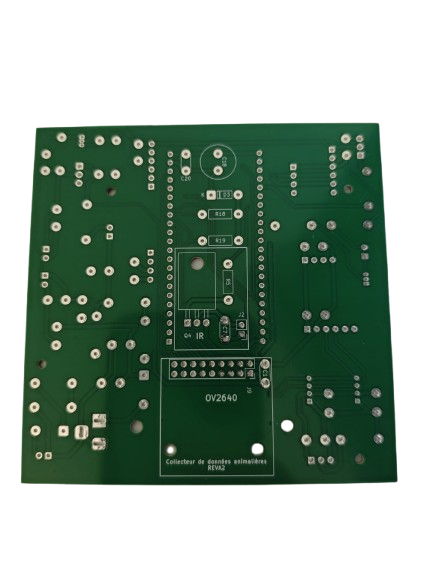
\includegraphics[width=\linewidth]{Images/WP1_2/Tache_8/PCB_BACK.png}
        \par\small Vue du bas du PCB après réception
    \end{minipage}
    \caption{Rendu final PCB après réception}
\end{figure}

\begin{figure}[H]
    \centering
    \begin{minipage}[t]{0.48\textwidth}
        \centering
        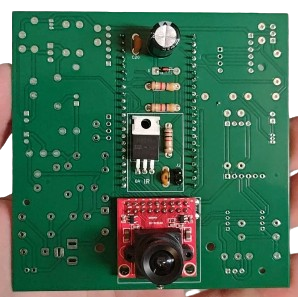
\includegraphics[width=\linewidth]{Images/WP1_2/Tache_8/PCB_BACK_APSOUD.png}
        \par\small Vue du bas du PCB après soudage
    \end{minipage}
    \hfill
    \begin{minipage}[t]{0.48\textwidth}
        \centering
        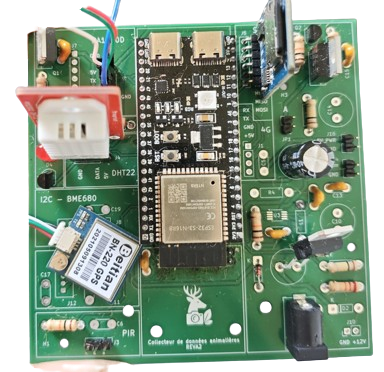
\includegraphics[width=\linewidth]{Images/WP1_2/Tache_8/PCB_TOP_APSOUD.png}
        \par\small Vue du haut du PCB après soudage
    \end{minipage}
    \caption{Rendu final}
\end{figure}

Après vérification de notre montage, nous avons remarqué deux problèmes majeurs, l'un étant plus grave que l'autre : 
\\

Le problème numéro 1 est que l'empreinte de la caméra était inversée. Il y a deux lignes de broches et, sur notre PCB, selon la manière dont nous voulions la positionner, elles étaient interchangées. Cela a eu pour conséquence qu'une fois la caméra soudée et le système mis sous tension, nous avons observé une chute de tension.
La solution que nous avons mise en place a consisté à dessouder la caméra et à mettre des câbles volants. Le PCB avait pourtant été prévu pour cela... dommage.
\\

Le deuxième problème concerne l'alimentation du PIR. Dans le schéma, une erreur s'est glissée et le PIR est connecté au 5V POWERUP, ce qui est incorrect ;
il devrait être connecté au 5V REGULATOR. Par conséquent, le PIR n'était pas alimenté et ne pouvait donc pas détecter les mouvements. 
La solution temporaire a été de le connecter au connecteur d'alimentation prévu pour d'autres modules, au cas où. 
\\

Malgré ces deux erreurs, il ne s'agit que d'erreurs mineures, ce qui rend tout de même notre PCB fonctionnel. Nous avons ainsi pu réaliser les tests de tension 
et de fonctionnement de notre système avec le PCB, ce qui constitue une grande réussite pour notre projet.
\\

\begin{figure}[H]
    \centering
    \begin{minipage}[t]{0.48\textwidth}
        \centering
        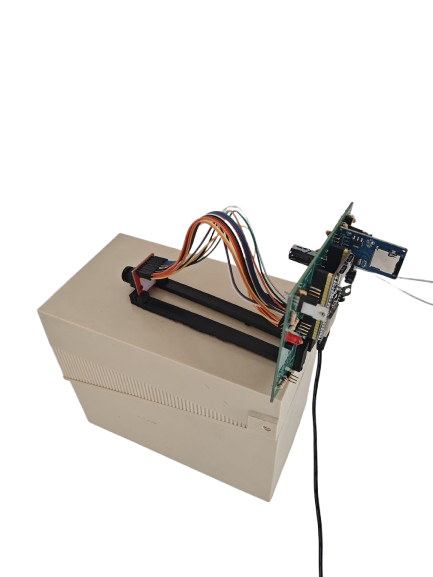
\includegraphics[width=\linewidth]{Images/WP1_2/Tache_8/Proto_Final.png}
        \par\small Prototype final avec le PCB soudé et fonctionnel
    \end{minipage}
    \hfill
    \begin{minipage}[t]{0.48\textwidth}
        \centering
        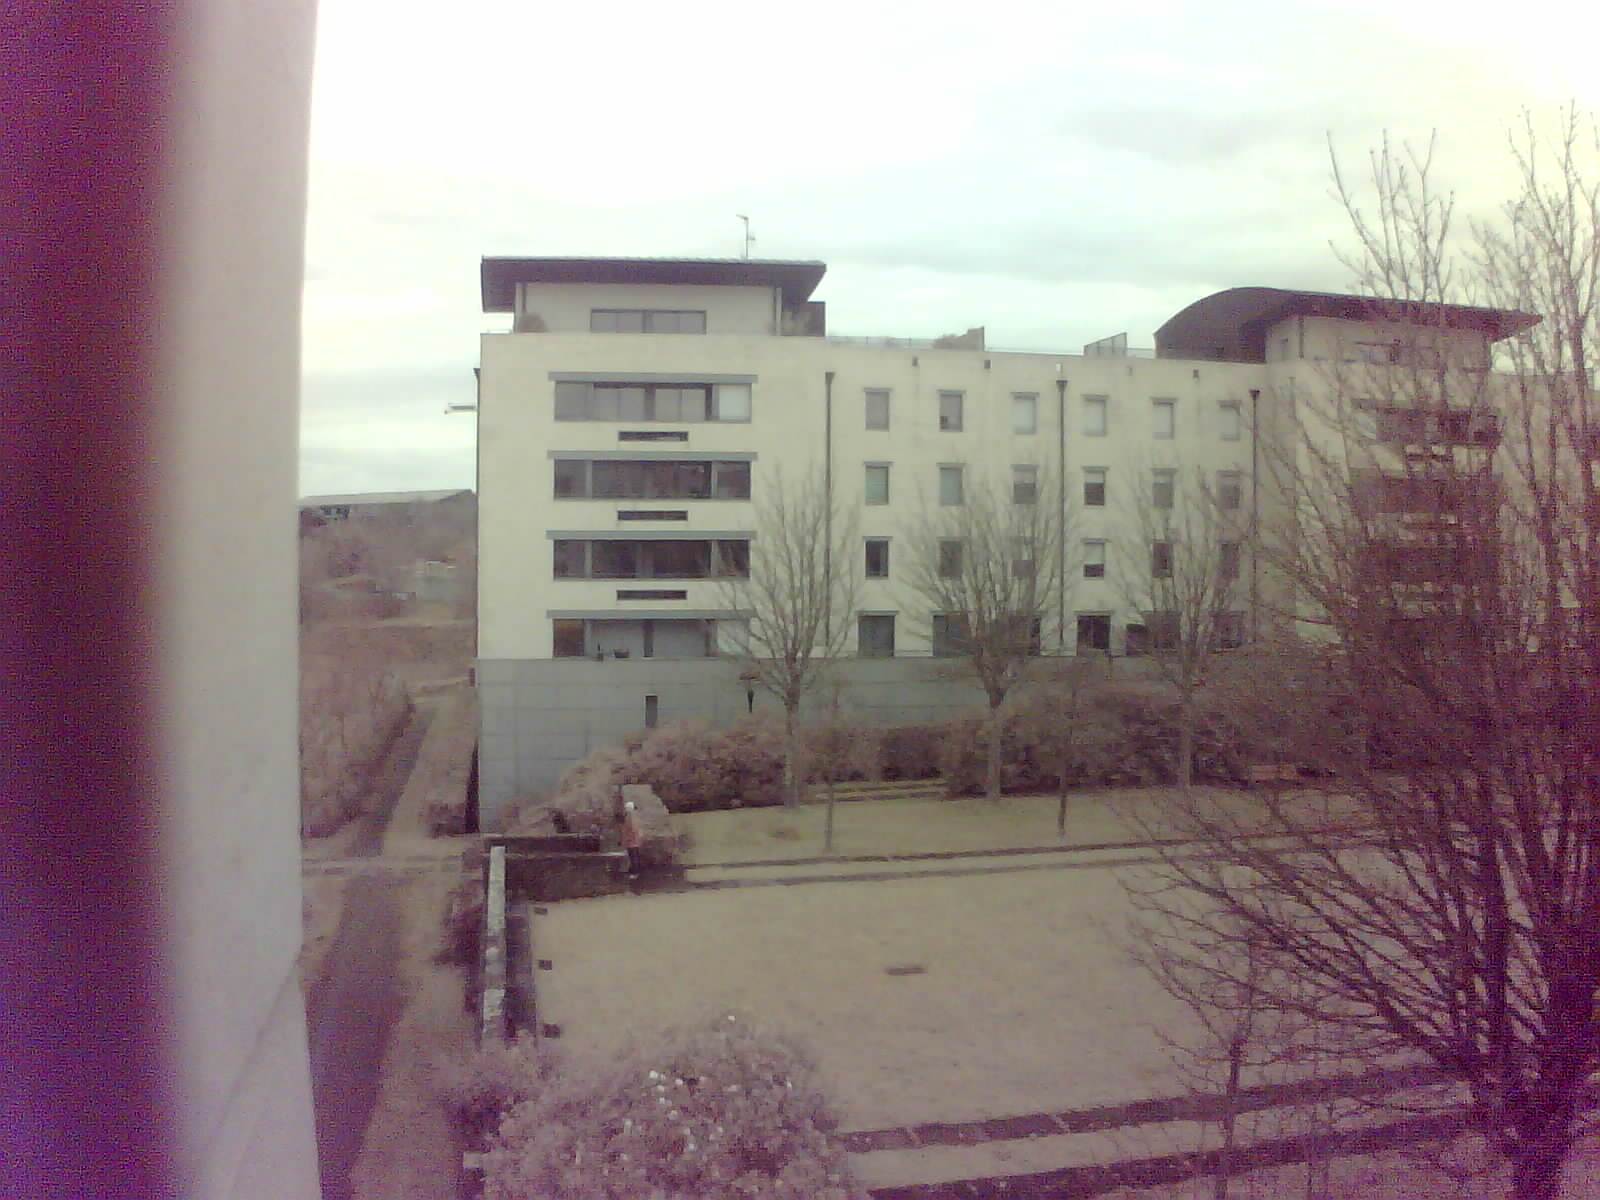
\includegraphics[width=\linewidth]{Images/WP1_2/Tache_8/Result.png}
        \par\small Vue du haut du PCB après soudage
    \end{minipage}
    \caption{Rendu final}
\end{figure}

\subsubsection{Synthèse du WP1.2}

Dans ce WP1.2 nous avons réalisé la partie de développement du module, qui correspond à la partie électronique et logicielle 
de notre projet. Nous avons réalisé un prototype fonctionnel de notre système, qui nous a permis de valider les différentes 
fonctionnalités de notre système, ainsi que de tester les différentes solutions envisagées pour la gestion de l'alimentation 
et de la consommation d'énergie.
\\

Nous avons aussi réalisé un schéma électrique de notre système, ainsi que la réalisation du PCB, ce qui était un objectif majeur.
\\

Sur le plan personnel je me suis beaucoup épanoui dans ce WP, j'étais au centre du Work Package, avec au début une sorte de mini pression
pour ne pas décevoir mon chef de projet, mais cela s'est plutôt bien déroulé.
\\

Le matériel a été le plus gros problème de ce WP, nous avons eu beaucoup de problèmes de commande, nous avons dû utiliser, ou même commander 
par nous-mêmes le matériel nécessaire pour la réalisation de notre projet, ce qui a engendré des retards dans notre planning,
mais nous avons réussi à faire face à ces problèmes et à avancer dans notre projet malgré tout.
\\



\subsection{WP 1.3 — Caméra (responsable : Xueying Xu)}

\subsubsection{Rappel des objectifs}

Le work package WP1.3 correspond au module caméra du système.

Son objectif principal est de permettre la prise d’images dans le cadre du piège caméra, afin de récupérer des données exploitables sur les animaux détectés.

Plus concrètement, les tâches associées sont :

\begin{itemize}
\item Capturer une image lorsqu’un signal de déclenchement est reçu (capteur ou commande)
\item Générer des images dans un format adapté, notamment le format JPEG
\item Assurer un fonctionnement en conditions de jour comme de nuit, avec un mode nocturne basé sur un éclairage infrarouge
\item Obtenir une qualité d’image suffisante pour permettre une observation correcte
\item Assurer que les images puissent être utilisées par les autres modules, en particulier le module MCU (WP1.2) et l’interface web (WP2.2)
\item Étudier l’influence de certains paramètres (résolution, distance, etc.) sur la qualité et la taille des images
\end{itemize}

Au début du projet, plusieurs solutions ont été testées (Raspberry Pi, ESP32-CAM) afin de valider le fonctionnement global. La solution matérielle finale étant traitée dans le WP1.2, cette partie se concentre surtout sur la gestion des images et leur format.

Dans ce contexte, nous avons mené une étude spécifique sur le choix du format d’image ainsi que sur son impact sur le système global. En particulier, le format JPEG a été analysé en lien avec la taille des données, la qualité de l’image et les contraintes de transmission. Parallèlement, nous avons également réalisé plusieurs tests afin d’évaluer l’influence de la résolution et des conditions de prise de vue sur le module caméra et la qualité de l’image.

\subsubsection{Solution envisagée}

Afin de répondre aux objectifs du WP1.3, une solution basée sur l’acquisition et la gestion d’images au format JPEG a été retenue.

Une phase de prototypage a d’abord été réalisée à l’aide de différentes plateformes (Raspberry Pi puis ESP32-CAM) afin de valider le principe de capture d’image et de transmission. La solution matérielle finale étant traitée dans le WP1.2, cette partie se concentre principalement sur le traitement des images.

La chaîne de fonctionnement mise en place est illustrée sur la figure ci-dessous. Elle comprend le déclenchement de la capture, l’acquisition de l’image, la génération d’une image compressée au format JPEG, puis son stockage temporaire avant exploitation par les autres modules du système.

\begin{figure}[H]
\centering
\begin{tikzpicture}[
    node distance=2cm,
    every node/.style={
        draw,
        rectangle,
        rounded corners,
        align=center,
        minimum width=3cm,
        minimum height=1cm
    },
    arrow/.style={->, thick}
]

\node (trigger) {Déclenchement};
\node (capture) [below of=trigger] {Capture de l'image};
\node (jpeg) [below of=capture] {Encodage JPEG};
\node (buffer) [below of=jpeg] {Stockage temporaire};
\node (output) [below of=buffer] {MCU (WP1.2) et modules WP2};

\draw[arrow] (trigger) -- (capture);
\draw[arrow] (capture) -- (jpeg);
\draw[arrow] (jpeg) -- (buffer);
\draw[arrow] (buffer) -- (output);

\end{tikzpicture}
\caption{Chaîne d’acquisition et de traitement des images du module caméra}
\end{figure}

\FloatBarrier

\paragraph{Choix du capteur OV2640}

Le capteur OV2640 a été retenu car il est bien adapté à une application embarquée de faible coût. Il est compatible avec l’ESP32 et permet de produire directement des images exploitables dans le système.

Son fonctionnement repose sur la conversion de la lumière captée par le capteur en données numériques. Ces données peuvent ensuite être traitées afin de générer une image compressée au format JPEG, qui sera récupérée par le microcontrôleur pour être stockée ou transmise.

Ce choix présente plusieurs avantages dans le cadre du projet :
\begin{itemize}
\item génération directe d’images JPEG ;
\item réduction de la charge de traitement côté microcontrôleur ;
\item taille de données plus adaptée à la transmission ;
\item bonne intégration dans une architecture embarquée.
\end{itemize}

\paragraph{Principe du format JPEG}

Le format JPEG repose sur une compression avec perte, ce qui permet de réduire fortement la taille des images. Son principe est de représenter l’image en séparant les informations les plus importantes de celles qui le sont moins pour l’œil humain.

D’un point de vue théorique, l’image est découpée en blocs, puis chaque bloc est transformé dans le domaine fréquentiel, généralement par une transformée en cosinus discrète (DCT). Les coefficients obtenus sont ensuite quantifiés : les composantes les moins importantes, souvent associées aux hautes fréquences, sont réduites ou supprimées. Cette étape permet de diminuer fortement la quantité de données à stocker ou à transmettre.

Dans notre cas, ce format est particulièrement intéressant car il permet de réduire la taille des données tout en conservant une qualité visuelle suffisante pour l’observation et l’exploitation des images dans le système global.

Par ailleurs, un fonctionnement en mode jour et nuit a été pris en compte. En conditions de faible luminosité, un éclairage infrarouge permet de maintenir la capture d’images.

\subsubsection{Tests et Validation}

Afin d’évaluer les performances de la chaîne d’acquisition d’image sur plateforme ESP32, nous avons réalisé une série de tests.

Tout d’abord, nous avons vérifié le format des images générées. Les résultats montrent que le module peut correctement générer des images au format JPEG, et que ces images peuvent être utilisées par les autres modules du système.

De plus, nous avons étudié l’influence de la résolution sur la taille des images. Les résultats montrent qu’avec l’augmentation de la résolution, la taille des images augmente également, passant de quelques kilooctets en basse résolution (QQVGA) jusqu’à environ 30 kB en haute résolution (XGA). Comme illustré sur la figure ci-dessous, une augmentation de la résolution entraîne une augmentation de la taille des images ainsi qu’un impact sur le temps de capture.

\begin{figure}[H]
\centering
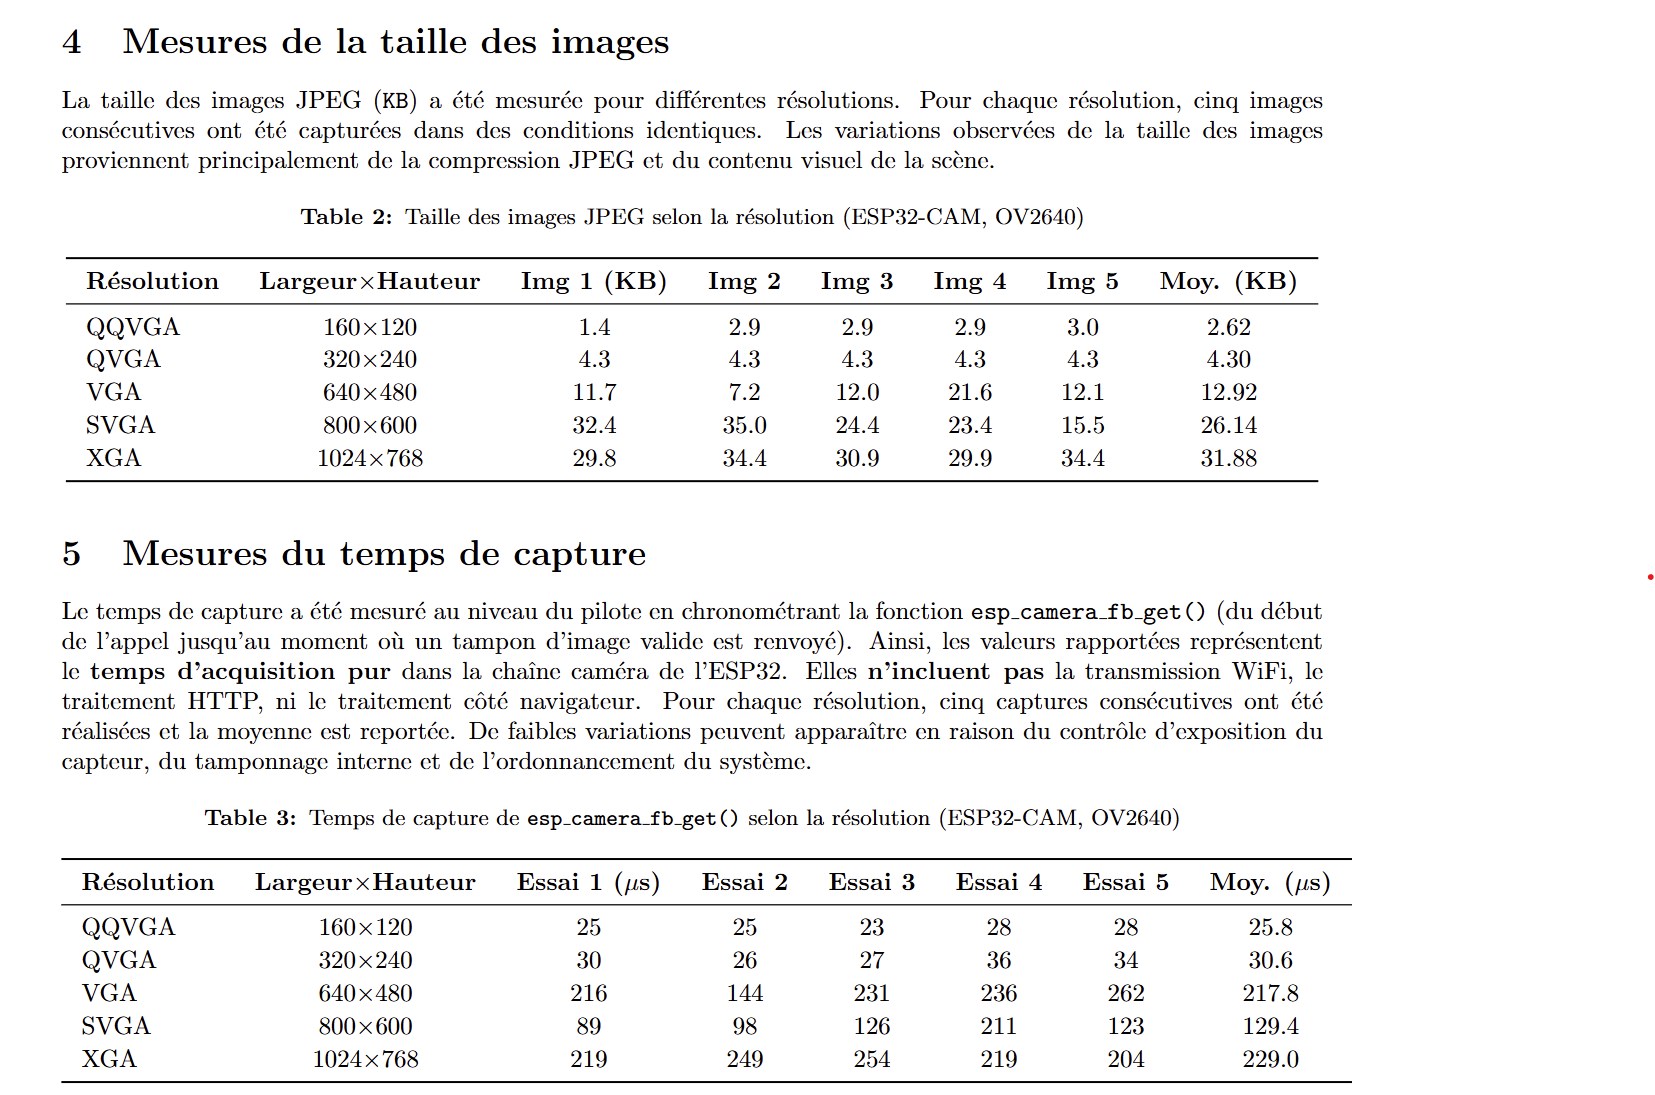
\includegraphics[width=0.85\textwidth]{mesures_camera.png}
\caption{Influence de la résolution sur la taille des images JPEG et le temps de capture}
\end{figure}

Nous avons également analysé le temps de capture des images. Les résultats montrent que le temps de capture est globalement faible, mais qu’il varie en fonction de la résolution. Cependant, la latence globale provient principalement de la transmission WiFi ainsi que du traitement côté client.

Enfin, nous avons testé la qualité des images à différentes distances de prise de vue. Les résultats montrent que la qualité est bonne à courte distance, mais qu’elle diminue progressivement lorsque la distance augmente.

Globalement, ces résultats montrent que le module caméra fonctionne correctement et qu’il répond aux besoins du projet en termes de qualité d’image et de transmission des données.

\FloatBarrier

\subsection{WP 1.4 — Conception et fabrication du boitier (responsable : Joris Menard)}
\subsubsection{Rappel des objectifs}
Détailler objectifs et liste des taches.
\subsubsection{Solution envisagé}
Travail théorique et recherches
\subsubsection{Tests et Validation}
Tests et validation de vos taches.

\subsection{WP bis — Transmission (responsable : Joris Menard)}
\subsubsection{Rappel des objectifs}
Détailler objectifs et liste des taches.
\subsubsection{Solution envisagé}
Travail théorique et recherches
\subsubsection{Tests et Validation}
Tests et validation de vos taches.

\subsection{WP 2.1 — Stockage distant (responsable : Davy Clark)}
\subsubsection{Rappel des objectifs}
Détailler objectifs et liste des taches.
\subsubsection{Solution envisagé}
Travail théorique et recherches
\subsubsection{Tests et Validation}
Tests et validation de vos taches.

\subsection{WP 2.2 — Interface web (responsable : Xueying Xu)}
\subsubsection{Rappel des objectifs}
Le work package WP2.2 correspond à l’interface web du système.
Son objectif principal est de permettre à l’utilisateur de consulter et gérer les données collectées par le piège caméra de manière simple et accessible via un navigateur web.
Plus concrètement, les tâches associées sont :
\begin{itemize}
\item Afficher les images capturées par le module caméra
\item Permettre un accès au système via une interface web (adresse IP / site)
\item Associer aux images certaines informations (date, heure, etc.)
\item Visualiser l’état du système (caméra, batterie, etc.)
\item Proposer différentes fonctionnalités (visualisation des images, gestion des caméras, journal système, etc.)
\item Offrir une interface claire et intuitive pour l’utilisateur
\end{itemize}
Cette interface constitue le lien entre le système embarqué et l’utilisateur final.

\subsubsection{Solution envisagé}
Travail théorique et recherches
\subsubsection{Tests et Validation}
Tests et validation de vos taches.

\subsection{WP 2.3 — Classification animalière par IA (responsable : Ewen Le Callet)}
\subsubsection{Rappel des objectifs}
Détailler objectifs et liste des taches.
\subsubsection{Solution envisagé}
Travail théorique et recherches
\subsubsection{Tests et Validation}
Tests et validation de vos taches.


\section{Bilan du projet}
\subsection{Bilan technique}
\subsection{Bilan personnel}

\section{Conclusion}

\clearpage
\section*{Bibliographie}
\addcontentsline{toc}{section}{Bibliographie}
\begin{thebibliography}{9}

\bibitem{PMBOK2021}
Project Management Institute,
\textit{A Guide to the Project Management Body of Knowledge (PMBOK Guide)},
7\textsuperscript{e} édition, 2021.


\end{thebibliography}

\clearpage
\appendix
\section*{Annexes}
\addcontentsline{toc}{section}{Annexes}
\section{Répartition détaillée des Work-Packages}
Cette annexe peut contenir un tableau de suivi des tâches par membre, avec les dates de début, d'échéance et le statut d'avancement.

\section{Exemples de données collectées}
Cette annexe peut présenter des exemples de relevés (température, horodatage, détection de mouvement), ainsi que des captures d'écran de l'interface web.

\end{document}